% !TEX program = lulatex
% !TEX encoding = UTF-8 unicode
\documentclass[11pt]{book}
\usepackage[utf8]{inputenc}	

\usepackage[left=2.75cm,right=2.75cm,top=2cm,bottom=3cm]{geometry}
\usepackage{style}
\thispagestyle{fancy}
\title{Fundamentals of digital systems}
\author{Arthur Herbette \\
Prof. Mirjana Stojilovic}

\begin{document}
\setcounter{section}{8}
\title{Fundamental of digital systems}
\maketitle
\thispagestyle{empty}
\tableofcontents
\thispagestyle{empty}
\listoflectures
Juste a little test
 %! TeX program = lualatex
\lecture{1}{2025-02-17}{Number Systems}{}
% !TeX root = main.tex

\chapter{Numbser Systems}
\section{Digital representations}
\begin{parag}{Introduction}
    \begin{itemize}
        \item In mathematics, a \important{tuple} is a finite ordered sequence of elements. 
        \begin{itemize}
            \item An \important{n-tuple} is a tuple of $n$ elements, where $n$ is a nonnegative integer
        \end{itemize}
        \item In a \important{digital representation}, a number is represented by an \important{ordered n-tuple}
        \begin{itemize}
            \item Each element of the n-tuple is called a \important{digit} 
            \item The n-tuple is called a \important{digit vector} (or string of digits)
            \item The number of digits $n$ is called the \important{precision} of the representation
        \end{itemize}
    \end{itemize}
\end{parag}
\subsection{Representation of nonnegative integers}
\begin{parag}{Integer Digit-Vector}
    \begin{itemize}
        \item \important{Digit-vector (string)} representing the integer $x$ is denoted by:
        \[X = (X_{n-1}, X_{n-2}, \dots, X_1, \overbrace{X_0}^{\text{zero-origin}})\]
        We see here that it is a leftward-increasing indexing
        \item \important{Least-significant} digit (also called low order digit): $X_0$
        \item \important{Most-significant} digit (also called high-order digit): $X_{n-1}$
    \end{itemize}
\end{parag}
\begin{parag}{Elements of a number System}
    \[X = (X_{n-1}, X_{n-2}, \dots, X_1, X_0)\]
    \begin{itemize}
        \item The number system to represent the integer $x$ consists of
        \begin{itemize}
            \item the number of \important{digits} n
            \item A set of numerical \important{values} for the digits
            \begin{itemize}
                \item if a \important{set of values for a digit} $X_i$ is $D_i$, the cardinality of $D_i$ is $|D_i|$
            \end{itemize}
            \item A rule of interpretation
            \begin{itemize}
                \item Mapping between the set of digit-vector values and the set of integers
            \end{itemize}
            \item \important{Set size}
            \begin{itemize}
                \item The set of integers is a finite set of at most $K$ elements
            \end{itemize}
        \end{itemize}
    \end{itemize}
    \begin{formule}
    \[K = \Pi_{i = 0}^{n-1} |D_i|\]
    \end{formule}
\end{parag}
\begin{parag}{Example: Decimal number system}
    \[X = (X_{n-1}, X_{n-2}, \dots, X_1, X_0)\]
    \begin{itemize}
        \item Number of digits $n$
        \begin{itemize}
            \item Can be any, but let us consider $n = 6 (e.g., 17, 9899, 676799, \dots)$
            \item Leading zeros are irrelevant
        \end{itemize}
        \item Digit set in decimal number system
        \begin{itemize}
            \item $D_i = \{0, 1, 2, \dots, 9\}$ of cardinality $10$
        \end{itemize}
        \item The correponding set size of $K$ is one million values, from $0$ to $K-1$
        \begin{itemize}
            \item $K = \prod_{i = 0}^{n-1} 10 = 10^6$
        \end{itemize}
    \end{itemize}
\end{parag}
\begin{parag}{(Non)Redundant Number systems}
    \begin{itemize}
        \item A number system is \important{nonredundant} if 
        \begin{itemize}
            \item ... each digit-vector represents a \important{different} integer
            \item E.g., the decimal system is nonredundant as every number is unique
        \end{itemize}
        \item Alternatively, a number system is \important{redundant} if ...
        \begin{itemize}
            \item ... there are integers represented by \important{more than one} digit-vector
        \end{itemize}
    \end{itemize}
\end{parag}
\begin{parag}{Weighted (Positional number systems}
    \begin{itemize}
        \item Most frequently used number systems are \important{weighted systems}
        \item The rule of representation:
        \[x = \sum_{i = 0}^{n-1} X_i W_i\]
        Where $W = (W_{n-1}, W_{n-2}, \dots, W_1, W_0)$ is the \important{weight-vector} of size $n$
        \item Equivalent formulation:
        \[x = X_{n-1}W_{n-1} + X_{n-2}W_{n-2} + \cdots + X_1W_1 + X_0 W_0\]
    \end{itemize}
\end{parag}
\begin{parag}{Example Decimal Number system}
    \begin{itemize}
        \item Weights are a power of $10$. Example:
        \begin{itemize}
            \item Digit Vector $X = (8, 5, 4, 6, 0, 3)$
            \item Weight vector $W = (10^5, 10^4, 10^3, 10^2. 10^1, 10^0)$
        \end{itemize}
    \end{itemize}
    $x = 8 \cdot 10^5 + 5 \cdot 10^4 + 4\cdot 10^3 + 7 \cdot 10^2 + 0 \cdot 10^1 + 3 \cdot 10^0$
    \\
    $x = 854703_{10}$
    \begin{itemize}
        \item When weights are of the format
        \begin{itemize}
            \item $W_0 = 1$ and 
            \item $W_i = W_{i-1}R_{i-1}, \; \; i \leq i \leq n-1$
        \end{itemize}
    \end{itemize}
    We have a \important{radix number system}
\end{parag}
\begin{parag}{Radix number system}
    \begin{definition}
        Radix number systems are weighted number system in which the weight vector is related to the \important{radix vector} $R = (R_{n-1}, R_{n-2}, \dots, R_1, R_0)$ as follows:
        \[W_0 = 1; \; W_i = W_{i-1}R_{i-1}, \; 1 \leq i \leq n-1\]
    \end{definition}
    \begin{itemize}
        \item Equivalent to
        \[W_0 = 1; \; W_i = \prod_{j=0}^{i-1} R_j\]
        \item E.g., in the decimal number system $W_0 = 1; W_i = \prod_{j = 0}^{i-1} 10$
    \end{itemize}
    \begin{subparag}{Fixed and Mixed-Radix number systems}
        \begin{itemize}
            \item In a \important{fixed-radix} system, all elements of the radic-vector have the same value \important{r (the radix)}
            \item The weight vector in a fixed-radix system:
            \[W = (r^{n-1}, r^{n-2}, \dots, r^2, r^1, 1)\]
            and the integer $x$ becomes 
            \[x = \sum_{i = 0}^{n-1} X_i \cdot r^i\]
        \end{itemize}
    \end{subparag}
    \begin{subparag}{Example}
        \begin{itemize}
            \item Characteristics of the decimal number system:
            \begin{itemize}
                \item Radix $r = 10$
                \item \textbf{Fixed-radix} system
            \end{itemize}
        \end{itemize}
    \end{subparag}
\end{parag}
\begin{parag}{Binary/Octal/Hexadecimal to/from Decimal}
I won't really go into the details here but the main thing to know is to convert from a system to one another (with the most famous ones)
\end{parag}
\subsubsection{Representation of signed Integers}
\begin{parag}{Sign-and-Magnitude (SM)}
    \begin{itemize}
        \item A signed integer $x$ is represented by a pair
        \[(x_s, x_m)\]
        where $x_s$ is the \important{sign} and $x_m$ is the \important{magnitude} (positive integer)
        \item Sign (positive, negative) is represented by a binary bariables 
        \begin{itemize}
            \item $0 \implies$ positive; $1 \implies $ negative
        \end{itemize}
        \item Magnitude can be represented as any positive integer
        \begin{itemize}
            \item In a conventional radix-r system, the range of n-digit magnitude is :
            \[0 \leq x_m \leq r^n - 1\]
        \end{itemize}
    \end{itemize}
\end{parag}

\lecture{2}{2025-02-20}{Arithmetic Operations with integers}{}
\section{Addition of unsigned Integers}
\begin{parag}{By hand}
    We use here the same principle as a classical addition by hand of decimal numbers : 
\end{parag}
    \begin{center}
    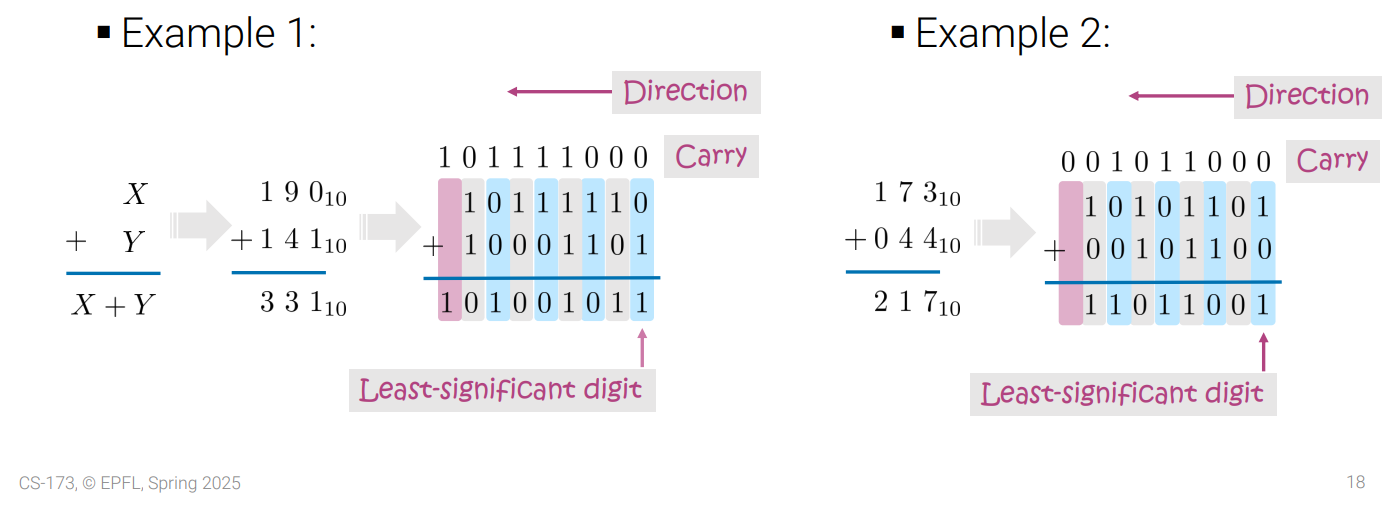
\includegraphics[scale=0.4]{Capture d’écran (112).png}
    \end{center}
\begin{parag}{How many Bits are needed}
    To represent the \important{sum of two $n$-bit unsigned numbers} we use \important{$n + 1$}
    \\
    For exemple the minimum space is when there are $0$ + $0$ which leads to : 
    \[s_{min} = 0 + 0 = 0\]
    and for the maximum : 
    \[s_{max} = (2^n - 1 ) + (2^n - 1) = 2\cdot 2^n -2 = 2^{n+1} - 2\]
    which makes it $n + 1$ bits for the sum.
    \begin{itemize}
        \item But we do not always have the extra bit in hardware
        \item When the magnitude of the result exceeds the largest representable value,  we say an \important{overflow} occurs and the result is incorrect.
    \end{itemize}
\end{parag}    
\subsection{Substraction of Unsigned Integers}
\begin{itemize}
    \item We use here the same idea as for decimal numbers : 
\end{itemize}
\begin{center}
    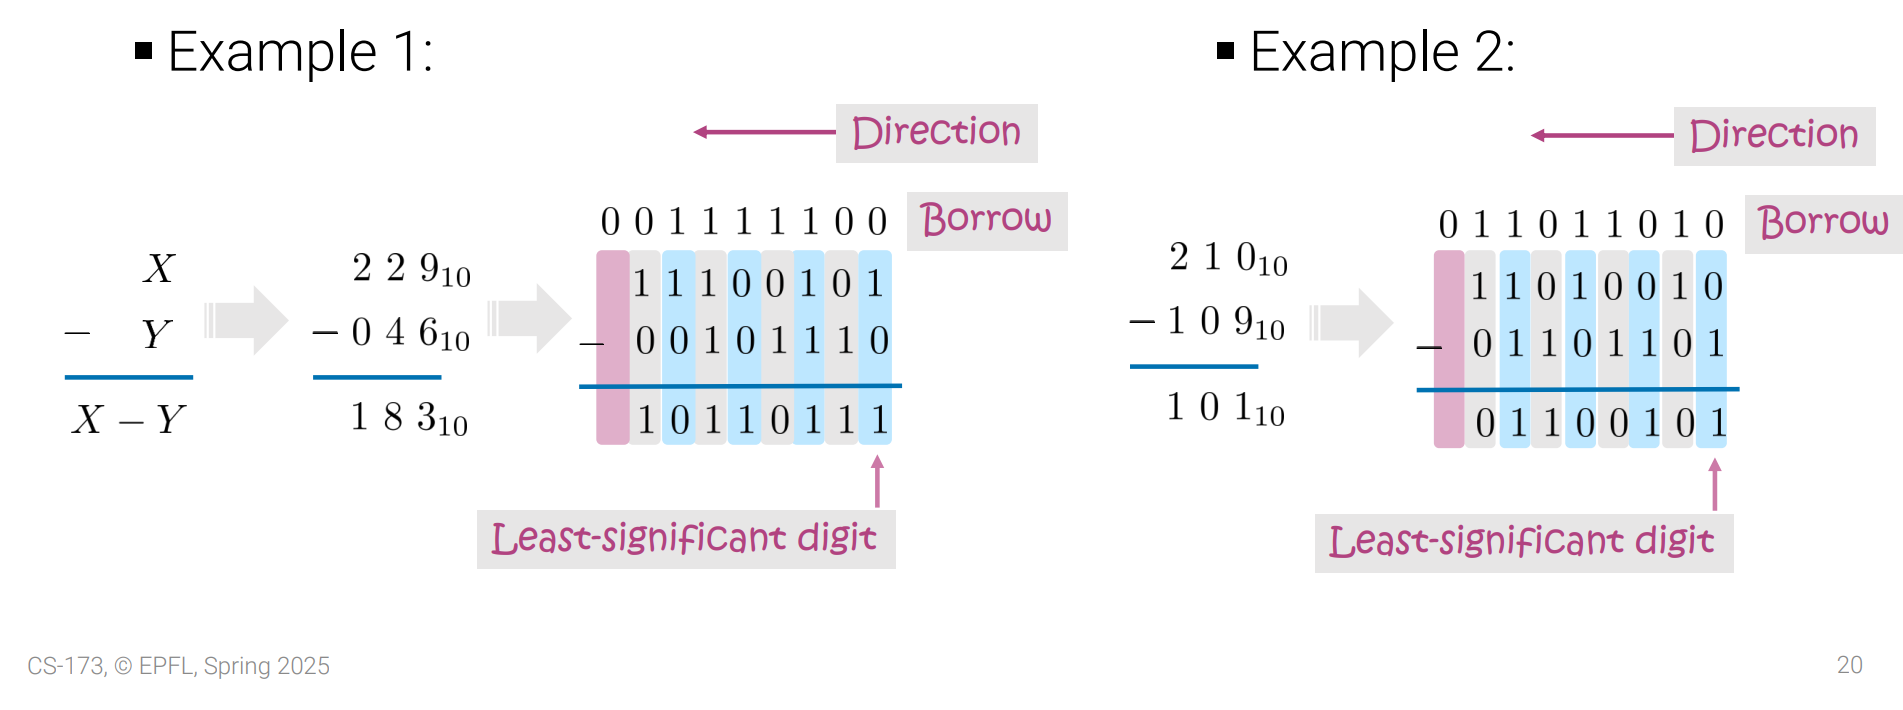
\includegraphics[scale=0.3]{Capture d’écran (113).png}
\end{center}
\begin{parag}{Negative result}
    \begin{itemize}
        \item Negative results cannot be represented using an unsigned system
        \item When trying to represent a value smaller than the minimu representable by the given number of bits $n$, an integer \important{underflow} occurs, and the result is incorrect.
    \end{itemize}
\end{parag}

\subsection{Two's Complement Addition/substraction}
\begin{parag}{Addition}
    We use here the same algorithm as for the unsigned numbers, and if the result exceeds the range, \important{overflow} occurs.
    \\
    To refresh how signes numbers works, for example $1000_2 = -8_{10}$ which is the "\textit{most negative}" number with $4$ bits. Then we add the right side of the number as positive integers like this:
    \[\underbrace{1}_{-8_{10}}\overbrace{010_2}^{2} = -6_{10}\]
    If we want to sum up $-5$ and $7$ for exemple:
    \begin{align*}
        1011 + 0111 \\
        \overbrace{1 + 1}^10\\
        \overbrace{1}^110 \\
        \overbrace{1}^1010 \\
        0010 = 2_{10}
    \end{align*}
    We use it as a clock : 
\end{parag}

\begin{center}
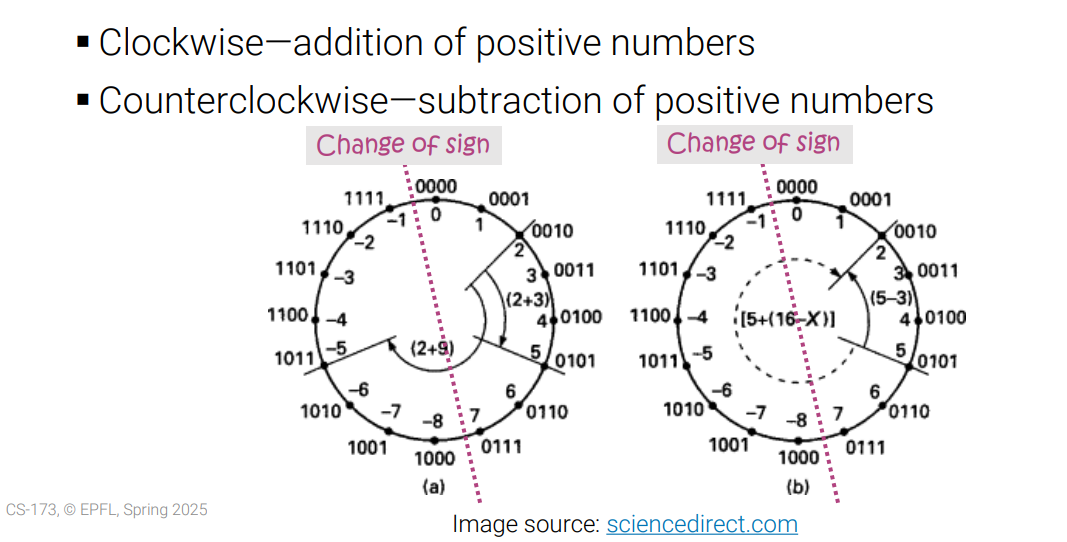
\includegraphics[scale=0.4]{Capture d’écran (114).png}
\end{center}

\begin{parag}{The preferred representation in digital Systems}
    \begin{itemize}
        \item If we start with the smallest (most negative) number $1000_2 = -8_{10}$ and count up all succesive numbers up to $0111_2 = 7_{10}$ can be obtained by adding $1$ to the previous one :
        \begin{itemize}
            \item The result will always be correct as long as the range is not exceeded
            \item Simple operation
            \item Not as simple for sign and magnitude
            \item Good for hardware implementation
            \begin{itemize}
                \item \important{Win-win}: the same hardware can perform the addition of unsigned numbers
            \end{itemize}
        \end{itemize}
    \end{itemize}
\end{parag}
\begin{parag}{Overflow Detection rules}
    \begin{itemize}
        \item Same algorithm as for the unsigned numbers
        \item If the result exceeds the range, \important{overflow} occurs
        \item \important{Overflow detection rules}
        \begin{itemize}
            \item If the signes of the two numbers are the same but different from the sign of the sum, the overflow occured
            \item Alternative formulation: if $c_{in}$ into  $c_{out}$ out of the sign position are different, the overflow occured
            \item Adding two numbers of different signs never produces an overflow
        \end{itemize}
    \end{itemize}
\end{parag}

\subsection{Binary multiplication}
\begin{parag}{How}
    We use the same "\textit{algorithm}" that the one we use by hand. For a binary representation:
    \begin{align*}
        X\cdot Y &= X \cdot \sum_{i=0}^{n-1} Y_i\cdot 2^i \\
        &= \sum_{i=0}^{n-1}X\cdot Y_i\cdot 2^i \\
        &= Y_{n-1} \cdot \underbrace{X \cdot 2^{n-1}}_{\text{Mulit Left-shifted by }n-1} + \cdots + Y_2\overbrace{X \cdot 2^2}^{\text{Mult Left shifted by }2} + Y_1\cdot X \cdot 2^1 + Y_0 \cdot X \cdot 2^0
    \end{align*}
\end{parag}
\begin{parag}{How many bits}
    \begin{theoreme}
        Given a $n$-bits intger and a $m$-bits intgers, there product can at most require $n + m$ bits.
    \end{theoreme}
    \begin{framedremark}
        We can see the multiplication as a sequence of $m$ additions with an $n$-bit number.
    \end{framedremark}
\end{parag}
\begin{parag}{Two's Complement multiplication}
    Recall of a value in two's complement (signed byte) : 
    \[x = -X_{n-1}2^{n-1} + \sum_{i = 0}^{n-2}X_i2^i\]
    \begin{itemize}
        \item Inspired by the previous algorithm:
        \begin{align*}
            X \cdot Y &= X \cdot (-Y_{n-1}\cdot 2^{n-1}) + X \sum_{i=0}^{n-2}Y_i\cdot 2^i \\
            &= -X\cdot Y_{n-1}\cdot 2^{n-1} + \sum_{i=0}^{n-2}X \cdot Y_i\cdot 2^i \\
            &= -Y_{n-1}\cdot X \cdot 2^{n-1} + Y_{n-2}\cdot X \cdot 2^{n-2} + \cdots + Y_2\cdot X\cdot 2^2 + Y_1\cdot X\cdot 2^1 + Y_0\cdot X\cdot 2^0
        \end{align*}
    \end{itemize}
    \begin{framedremark}
        Let us not forget the sign-extend the partial result
    \end{framedremark}
    For this only $n + m$ bits are kept; any higher-order bits are discarded. (that the "\textit{reason}" how $-5\cdot -3 = 15$
\end{parag}
\begin{parag}{Sign-Magnitude and Two's Complement}
    I juste want to underline the difference between those two representation. 
    \begin{subparag}{Sign Magnitude}
        In the Sign magnitude representation with $n$ bits, we use the \important{most significant bit} (MSB) to use it as a sign:
        \begin{itemize}
            \item $0$ for positive numbers
            \item $1$ for negative numbers
        \end{itemize}
        The remaining bits represent the absolute magnitude of the number:
        \\
        To write $5$ in a $4$-bits number, we use $0101_2 = +5_{10}$
        \\
        To write $-5$ in a $4$-bits number, we use $1101_2 = -5_{10}$
        \\
        We see here that it is very intuitive and mirrors human notation with a sign.
    \end{subparag}
    \begin{subparag}{Two's Complement Representation}
        Here, there is two point of view the one introduce in the course is to see it as a clock, in a clockwise (le sens des aiguilles d'une montre) it is positive, and unclockwise (dans le sens contraire à celui d'une montre) it is negative and begin. The negative also start at $-1$ but the bit to represent $-1$ is $1111_2$ which is just on the left.
        \\
        The other way is to see it as the most significant bit (MSB) as negative, $1000_2 = -8$ and the rest of the bits being positive. To write $-5$ you have to write it as $-8 + 3 = -5$ which goes to $1011_2 = -5_{10}$
        \\
        The pros for this notation is that there is only one representation for $0$ where there is two for the other ($1000 = 0000 = 0)$, The arithmetic operation are easier because we don't have to carry a sign everywhere and it is mor efficient in hardware implementation.
    \end{subparag}
\end{parag}    
\begin{figure}[h]
\centering
    \caption{Comparison table}
    \begin{tabular}{|c|c|c|}
    \hline
    Feature & Sign-Magnitude & Two's complement \\
    \hline
    \hline
     $-5_{10} $ & $1101$   &   $1011$ \\
     \hline
        Zero representation  & $0000 (+0)$ and $1000 (-0)$ & $0000$ \\
        \hline
        Range ($4$-bit) & $[-7, 7]$ & $[-8, +7]$ \\
        \hline
        
    \end{tabular}
    
    \label{fig:enter-label}
\end{figure}
    
    

% !TeX program = lualatex
\lecture{3}{2025-02-24}{Fractional (Nointeger) Number}{}


\section{Fractional number}
\subsection{Fixed-Point Representation}
\begin{parag}{General Format}
    \begin{definition}
        Fixed-Point Numbers are:
        \begin{itemize}
            \item Integers
            \[I = -N, \dots, N\]
            \item Rational numbers ("\textit{binary}" rationals) of the form:
            \[x = \frac{a}{2^f}\]
            where $a \in I$ and $f$ positive integer
        \end{itemize}
    \end{definition}
    The fixed-point representation of a number $x$ consists of integer $x_{int}$ and fraction $x_{fr}$ components represented by $m$ and $f$ digits, respectively:
    \[x = x_{int} + x_{fr}\]
    \begin{definition}
        Digit-vector representation: 
        \[X = (X_{m-1}X_{m-2}\dots X_1X_0\underbrace{.}_{\text{Radix point}}X_{-1}X_{-2}\dots X_{-f})\]
        \begin{itemize}
            \item For \important{unsigned} numbers : 
            \[x = \sum_{i  = -f}^{m-1}X_i2^i\]
            \item For \important{signed} number in two's complement: 
            \[x = -X_{m-1}2^{m-1} + \sum_{i = -f}^{m-2}X_i2^i\]
        \end{itemize}
    \end{definition}
\end{parag}
\subsection{Radix point}
\begin{parag}{Separator between the integer and fractional parts}
    \[X = (X_{m-1}X_{m-2}\dots X_1X_0\underbrace{.}_{\text{Radix point}}X_{-1}X_{-2}\dots X_{-f})\]
    \begin{itemize}
        \item The position of the radix-point is assumed to be fixed
        \begin{itemize}
            \item Hence the name fixed-point
        \end{itemize}
        \item If the radix point is not shown, it is assumed to be to the right of the least significant digit (i.e, no fractional part)
        \begin{itemize}
            \item In that case, the number is an integer
        \end{itemize}
        \item Also known as decimal point, binary point, etc$\dots$
    \end{itemize}
\end{parag}
\begin{center}
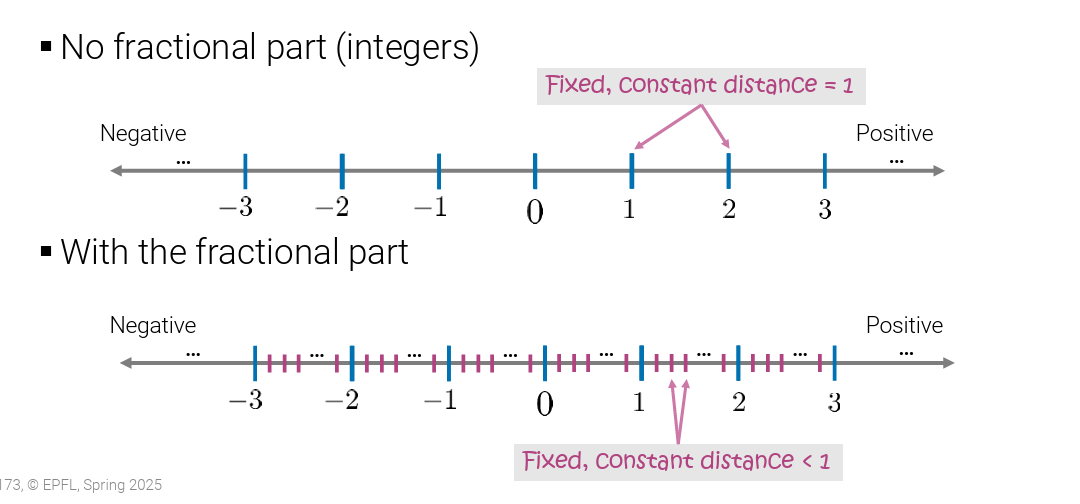
\includegraphics[scale=0.5]{Screenshot 2025-02-24 131346.png}
\end{center}

\
\begin{parag}{Example}
    \begin{itemize}
        \item Decimal number system and $m = 5, f = 5$
        \item Example decimal digit vector : 
            \begin{itemize}
                \item $X = (10077.01690)$
                \item $ x = 1 \cdot 10^4 + 7 \cdot 10^1 \cdots  + 0,009$
            \end{itemize}
        \item Most negative (min):
            \begin{align*}
                x_{min} = -99999.99999 = -99999 \frac{99999}{10^5}
            \end{align*}
            
        \item Largest number (max, positive):
            \begin{align*}
                x_{max} = +99999.99999 = +99999 \frac{99999}{10^5}
            \end{align*}

            
    \end{itemize}
    
\end{parag}



\begin{parag}{Fixed-point Representation}
    \begin{itemize}
        \item Given an unsigned fixed-point binary format $m = 3, f = 4$
            \begin{itemize}
                \item and an example binary digit vector:
                    \begin{align*}
                        X = (101.0111)
                    \end{align*}
                    
            \end{itemize}
        \item Q: Find the equivalent decimal number:
            \begin{align*}
                X = (101.0111); x = 2^2 + 2^0 + 2^{-2} + 2^{-3} + 2^{-4} = 5.4375
            \end{align*}
    \end{itemize}
    \begin{subparag}{Example}
        With sign-and-magnitude and $m = 5, f = 3$, Example of a binary digit vector:
        \begin{align*}
            X = (10101.110);\\
            x = -(4 + 1 + 0.5 + 0.25) = -5.75
        \end{align*}
        Therefore, The most negative number can be
        \begin{align*}
            x_{min} = 11111.111_2 = -15 \frac{7}{8}
        \end{align*}
        On the other hand, the largest number:
        \begin{align*}
            x_{max} = 01111.111 = 15 \frac{7}{8}
        \end{align*}
    \end{subparag}
    \begin{subparag}{Two's complement}
        With two's complement the work is the same as usual (the first digit is negative):
        \begin{align*}
            X =  (1010.1101); \\
            x = -8 + 2 + 0.5 + 0.0625 = -5.1875
        \end{align*}
        Here the most negative number is $x_{min} = 1000.0000_2 = -8$ and the largest one is $x_{max} = 0111.1111_2 = 7 \frac{15}{16}$
        
    \end{subparag}
\end{parag}
    \section{Concepts of finite precision math}
    \begin{parag}{Precision}
    \begin{definition}
        The precision is the maximum number of non-zero bits
    \end{definition}
    For example if we have $X = (X_{m-1}X_{m-2} \dots X_1 X_1 . X_{-1}X_{-2} \dots X_{-f}$ then, the precisions is the sum of $f$ and $m$:
    \begin{align*}
        \text{Precisions}(x) = m + f
    \end{align*}
    
    
    \end{parag}
   \begin{parag}{Resolution}
       \begin{definition}
           The resolution is the smallest possible difference between two consecutive numbers
       \end{definition}
       For example if a number as $f = 5$ (5 digits for is fractional part) then we know that the smallest possible difference between the number is $ \frac{1}{2^5} = \frac{1}{32}$ , for integer ($f = 0$) the resolution is $ \frac{1}{2^0} = 1$
   \\
   However, in the general case:
   \begin{align*}
       \text{Resolution(x)} = 2^{-f}
   \end{align*}

   
   \end{parag}
    
\begin{parag}{Rang}
    \begin{definition}
        The range is the difference between the most positive and the most negative number representable.
    \end{definition}
    For example with \important{two's complement}
    \\
    If we take, $m = 5, f = 3$, we compute $x_{max} = \sum_{i=-f}^{m-2}2^i = 15 \frac{7}{8}$, $x_{min} = -2^{m-1} = -16$. Then, the range is equal to $x_{max} - x_{min} = 31 \frac{7}{8}$
\\
In the general case, for fixed point and two's complement:
\begin{align*}
    \text{Range}(x) = x_{max} - x_{min} = \sum_{i-=f}^{m-2} 2^i - (-2^{m-1})
\end{align*}
\end{parag}
    \subsection{Accuracy}
    \begin{parag}{definition}
    \begin{definition}
        The accuracy is the magnitude of the maximum difference between a \textbf{real} value and its representation.
    \end{definition}
    
    The worst case (max difference) occurs for a real value exactly in the middle between two subsequent representable numbers (the real value lays between two equaly distant representation).
    \\
    In the general case = 
    \begin{align*}
        \text{Accuracy}(x) = \frac{ \text{Resolution} (x)}{2}
    \end{align*}    
    \end{parag}
    \begin{parag}{Dynamic Range}
        \begin{definition}
            The dynamic range is the \textbf{ratio} of, the maximum \textbf{absolute} value representable and the minimum positive value absolute (i.e nonzero) value representable.
        \end{definition}
        If we take the two's complement, with $m = 5, f=3$ then the maximum absolute value is $- -2^4 = 16$. For the minimum positive value we have $2^{-3} = \frac{1}{8}$. \\
    The dynamic range is said $ = \frac{x_{max}}{x_{min}} = 128$
In the general case, for fixed-point and two's complement:
\begin{align*}
    \text{Dynamic Range}(x) = \frac{2^{m-1}}{2^{-f}} = 2^{m-1 + f}
\end{align*}
\begin{subparag}{Personal remark}
    You can see as the \textit{size} of all the representable value divided by $2$, $128$. We have here $8$ bits which means that we have $2^8$ possible value which goes exactly to $256$.
\end{subparag}

        
    \end{parag}
    
\subsection{Floating-Point Number representation}
\begin{parag}{Floating-Point (FP) Representation}
    As with any other number representation in a digital system, $FP$ representation is encoded in a finite number of bits. It represents only a \important{finite subset} of the \important{infinite set} of real numbers.
    \\
    A real number that is \important{exactly} represented is called a \important{floating-point (FP) number}. All other real number either fall out of range (overflow or underflow) or are represented by $FP$ numbers that approximate their value. The process of approximation is called \important{roundoff} and produces a \important{roundoff error}.
    

\end{parag}

    \begin{parag}{Significand, Exponent, Base}
        $FP$ representation consists of two components : 
        \begin{itemize}
            \item the signed \important{significand} (also called \important{mantissa}) $M^*$
            \item the signed \important{exponent} $E$
                \begin{align*}
                    x = M^* \times b^E
                \end{align*}
                where $b$ is a constant called the \important{base}
                
        \end{itemize}
        Reminds us of the usual scientific notation, base $10$ :
        \begin{align*}
            +35200 = \underbrace{3.52}_{ \text{Coefficient}} \cdot 10^{+4} \; \; \; -0.099 = -9.9 \cdot \overbrace{10^{-2}}^{\text{Exponent}} 
        \end{align*}
        
    
    \end{parag}
    
    \begin{parag}{Benefits of Floating-Point}
        Consider $32$ bit two's complement signed integers:
        \begin{align*}
            \text{Dynamic Range}_1(x) = \frac{x_{max}}{x_{min}} = \frac{2^{32-1}}{2^0} = 2^31 \approx 2 \cdot 10^9
        \end{align*}
        New, let's consider alors a $32$ bit but floating-point number, with $24$-significand in sign and magnitude and $8$-bits exponent in two's complement.
        \begin{align*}
            \text{Dynamic Range}_2(x) = \frac{x_{max}}{x_{min}} = \frac{(2^{23}-1) \cdot 2^{2^{(8-1)}-1}}{2^0 \cdot2^{-2^{8-1}}} = (2^{23} - 1) \cdot2^{255} \approx 5 \cdot 10^{83}
        \end{align*}
        We can see here that the dynamic range increase a lot by a factor of $ \approx 10^{74}$
        
    
    \end{parag}
    
    \begin{parag}{Benefit}
        We can also see the benefits the resolution which also reduces of for example when taking a $32$-bits with $8$ fractional bits (fixed-point) and on the other side, $24$ bits significand in sign and magnitude and $8$ bit exponent in two's complement. If we compute each resolutions:
        \begin{align*}
            \text{Resolution}_1 (x) &= 2^{-8} = 0.00390625 \\
            \text{Resolution}_2(x) = 2^0 \cdot2^{-2^{(8-1)}} = 2^{-2^7} = 2^{-128}
        \end{align*}
        If we compute the ratio:
        \begin{align*}
            \frac{ \text{Resolution}_2(x)}{ \text{Resolution}_1(x)} = \frac{2^{-128}}{2^{-8}} = 2^{-120} \approx 7.523 \cdot 10^{-37}
        \end{align*}
        
    
    \end{parag}
   \subsection{Significand: Sign-and-Magnitude}
    
    \begin{parag}{Floating-Point Representation}
        Today, the most used representation for significand is sign and magnitude because it simplifies multiplication in hardware. 
        \\
        The floating-point representation becomes:
        \begin{align*}
            x = (-1)^S \times M \times b^E
        \end{align*}
        Where $S \in \{0, 1\}$ is the \important{sign} and $M$ is the \important{magnitude} of the signed significant
    \begin{framedremark}
        In the rest of the lecture, we assume significand is always represented in sign-and-magnitude.
    \end{framedremark}
    
    \end{parag}
    
    \begin{parag}{Digit vector}
        Many digit vectors are conceivable,  but we focus on the following:
        \begin{align*}
        X = ( \underbrace{SE_{m-1}}_{ \text{Sign}E_{m-2} \dots E_1 E_0 M_{n-1}M_{n-2} \dots M_0}
        \end{align*}
        Where $E_i$ is the exponent and $M_i$ is the magnitude.\\
        There is $(n+1)$ bit significand in \important{sign and magnitude} and $m$ bit exponent.
        
    
    \end{parag}
   \begin{parag}{Redundant}
       In the most general case, the representation: 
       \begin{align*}
           x = (-1)^S \times M \times b^E
       \end{align*}
       is redundant. Sign and magnitude is redundant, Multiple magnitude and exponent combinations can give the same number.
       \\
       \begin{subparag}{Example}
           If we take for example:
           \begin{align*}
               (1010)_2 \times 2^{-2} = 10 \times 2^{-2} = 2.5\\
               (0101)_2 \times 2^{-1} = 5 \times 2^{-1} = 2.5 \\
               (1.01)_2 \times 2^1 = 1.25 \times 2^1 = 2.5
           \end{align*}
           Floating-point representation is \important{redundant} \important{unless it is normalized}!
           \\
           If we take a magnitude that is \important{normalized}:
           \begin{align*}
               1 \leq M < 2
           \end{align*}
           Then: \begin{align*}
               1010.1000_2 = 1.0101_2 \times 2^3 = 10.5 \\
               -(0.00000011)_2 = -1.1_2 \times 2^{-7} = -0.01171875
           \end{align*}
          \begin{framedremark}
              Juste to be clearer, the normalized one here, is $1.0101_2 \times 2^3$ and $-1.1_2 \times 2^{-7}$. 
              \\
              For example let put $20_{10}$ normalized.
              \\
              First, $20_{10} = 10100_2$, however $ 1 \leq M < 2$, which leads us to: $1.0100_2 \times 2^4$. The $M$ being between $1$ and $2$ doesn't mean that the decimal number has a $1, \dots$.
          \end{framedremark}
       \end{subparag}
       
   
   \end{parag}
    
   \begin{parag}{Hidden Bit and Fraction}
       As the significand is normalized, the first digit of the magnitude is \important{always} binary $1$. If something is always the same, it can be omitted (saving precious bits)\\
       The first digit of the significand is omitted and called \important{hidden bit}. \\
       The binary point is assumed to the right of the hidden bit. The represented part of the significand is called \important{fraction F}.
   
       \begin{subparag}{Example}
           \begin{align*}
               \overbrace{101.001_2}^{ \text{unormalized significand}} \times 2^{-4}  = \underbrace{1.01001_2}_{ \text{Normalized significand}} \times 2^{-2} = \overbrace{.01001_2}^{ \text{hidden is not represented}} \times 2^{-2}
           \end{align*}
           
           
       \end{subparag}
   \end{parag}
   \begin{parag}{Summary}
       \begin{itemize}
           \item Common significand representation is the following:
               \begin{itemize}
                   \item Sign-and-magnitude
                   \item Normalized
                   \item One hidden bit
               \end{itemize}
           \item Corresponding significand value becomes:
               \begin{align*}
                   (-1)^S \times (1 + \sum_{i=1}^n M_{n-1} 2^{-1})
               \end{align*}
               
       \end{itemize}
   
   \end{parag}
   
      \section{Exponent}
      \begin{parag}{Exponent}
          Exponent needs to be signed
          \begin{itemize}
              \item \important{Positive} for representing very large numbers ( \important{large absolute} value)
              \item \important{Negative} for representing very small numbers ( \important{small absolute} value)
          \end{itemize}
      
      \end{parag}
      
      \begin{parag}{Biased representation}
          Exponent can take any signed representation we know but there is one particular representation, called \important{biased}, which simplifies comparing two $FP$ numbers in hardware.
          \\
          Biased representation of a digit vector $X = (X_{n-1} \dots X_1 X_0)$
          \begin{align*}
              x = \sum_{i=0}^{n-1} X_i 2^i - B
          \end{align*}
          
          Typically, the bias equals $B = 2^{n-1} - 1$
      
      \end{parag}
     \begin{parag}{Biased representation, Cntd.}
         Where's the catch?
         \begin{itemize}
             \item Resulting number are sorted just like unsigned integers but cover both the positive and negative numbers
             \item efficient hardware (superior to two's complement)
             \item Min exponent is represented as all zeros
             \begin{itemize}
                 \item $FP$ zero can be represented as all zeros (significand and exponent)
             \end{itemize}
         \end{itemize}

     
     \end{parag}
      
\subsubsection{Summary}
\begin{parag}{Exponent}
    \begin{itemize}
        \item Common representation of an -$m$ bit exponent is biased with base $B = 2^{m-1}-1$
        \item For the binary digit vector:
            \begin{align*}
                X = (SE_{m-1}E_{m-2} \dots E_1E_0 . M_{n-1}M_{n-2} \dots M_0)
            \end{align*}
            this biased exponent \textbf{value} becomes : 
            \begin{align*}
                e = \sum_{j=0}^{m-1} E_j 2^j - (2^{m-1} - 1)
            \end{align*}
            
    \end{itemize}

\end{parag}
\begin{parag}{Floating point format}
    There could be many floating point formats, but we will often assume:
   \begin{itemize}
       \item $(n+1)$-bit significand 
       \item Sign and magnitude
       \item Normalized, one hidden bit
   \end{itemize}
   \begin{itemize}
       \item $m$-bit exponent
           \begin{itemize}
               \item Biased, $B = 2^{m-1} -1$
           \end{itemize}
   \end{itemize}
   \begin{align*}
       X = (SE_{m-1}E_{m-2} \dots E_1 E_0 . M_{n-1} M_{n-2} \dots M_0)
   \end{align*}
   \begin{align*}
       x = (-1)^S \times (1 + \sum_{i=1}^n M_{n-i}2^{-i}) \times 2^{\sum_{j=0}^{m-1} E_j 2^j - (2^{m-1}-1)}
   \end{align*}
   
   

\end{parag}

    \section{Rounding}
    The result of a floating-point operation is a real number that, to be represented exactly might require a significand with an infinite number of digits.\\
    To obtain a representation close to the exact result, we perform what is called \important{rounding}
    \begin{parag}{Rounding modes}
        Various rounding modes exist
        \begin{itemize}
            \item Round to \important{nearest}, to \important{even} when \important{tie}
            \item Round towards \important{zero} (truncate)
            \item Round towards plus or towards minus \important{infinity}
        \end{itemize}
        Consider the real number $x_{real}$ and the consecutive floating-point number $F_1$ and $F_2$ \text{ such that }$F_1 \leq x_{real} \leq F_2$, we round it like always (normal definition)
      
    \end{parag}
    
    
    \subsection{IEE Standard 754}
        \begin{parag}{$FP$ format in IEEE 754}
            Exactly what we described
            \begin{itemize}
                \item $(n+1)-$bit significand
                    \item Sign and magnitude, Normalized, one hidden bit
                    \item $m$-bit exponent 
                        \begin{itemize}
                            \item Biased $B = 2^{m-1} - 1$
                        \end{itemize}
            \end{itemize}
            \begin{align*}
                X = (SE_{m-1}E_{m-2} \dots E_1E_0 . M_{n-1}M_{n-2} \dots M_0)
            \end{align*}
    There is two types of formats: Basic and extended format:
    \begin{subparag}{Basic formats}
        \begin{itemize}
            \item Sign $S$ $1$ bit
            \item Exponent $E$: $8$ bits
            \item Fraction $F$: $23$ bits
        \end{itemize}
        The default rounding mode is to the nearest, to even when there is a tie.
    \end{subparag}
    \begin{subparag}{Double precision (64 bits)}
        \begin{itemize}
            \item Sign $S$: 1 bit
            \item Exponent $E$: $11$ bits
            \item Fraction $F$: 52 bits
        \end{itemize}
        
        
    \end{subparag}
    \begin{subparag}{How to convert fixed-point to IEEE 754}
        In order to do this, we need $5$ steps:
        \begin{enumerate}
            \item Normalize the fixed point representation by shifting the binary point to the right of leftmost
            \item The mantissa is the entire binary string after the binary point (the mantissa stores the fractional part after the leading $1$ which is \textbf{implicit}.
            \item Calculate the exponent bits by adding the bias of $127$ to the power of $2$
            \item Convert exponent to unsigned binary representation
            \item If the number is positive, the sign bit is zero, otherwise it is $1$.
        \end{enumerate}
        Let us see for example the number such as: $13_{10}.625$. \\
        Firstly, we convert it to binary
        \begin{align*}
            13.625_{10} = 1101.101_2
        \end{align*}
        Now we have to normalized the binary number:
        \begin{align*}
            1.101101 \cdot 2^3
        \end{align*}
        So:
        \begin{itemize}
            \item Mantissa: $1.101101$ (the leading $1$ is \important{implicit} in $IEEE$ $754$).
            \item Exponent: $3$ (since we moved the decimal point $3$ point left)
        \end{itemize}
        Then we compute the biased Exponent. In $IEEE\; 754$, we use a bias of $127$:
        \begin{align*}
            E = 3 + 127 = 130 \\
            130_{10} = 10000010
        \end{align*}
        We then drop the leading $1$ from the $1.101101$, fille the rest of the bit on the right:
        \begin{align*}
            1011010000000000000000000000
        \end{align*}
        Which is the mantassima. this leads finally to:
        \begin{align*}
        1\overbrace{10000010}^{ \text{Exponent}} \underbrace{10110100000000000000000000000}_{ \text{Mantissa}}
        \end{align*}
        Which in hexadecimal:
        \begin{align*}
            C16C0000
        \end{align*}
        A cool video to understand how to convert any number to $IEEE$ $754$ format:
        \begin{center}
            \url{https://www.youtube.com/watch?v=RuKkePyo9zk}
        \end{center}
        
        
        
        
        

        
    \end{subparag}
        \end{parag}
        
        \begin{parag}{Special Values}
            \begin{itemize}
                \item Floating-point \important{zero}: $E = 0, F = 0$
                    \begin{itemize}
                        \item The sign $S$ differentiates between positive and negative zero, Value $1.0 \times 2^{-B}$ is not represented.
                    \end{itemize}
                \item Positive and negative \important{infinity}
                    \begin{itemize}
                        \item Biased exponents all ones, $F = 0$
                       
                    \end{itemize}
                \item \important{NaN} (not a number)
                    \begin{itemize}
                        \item To represent results of invalid operations(for example, the square root of a negative number)
                        \item Sign $= 0$ or $1$ biased exponents all ones, $F \neq 0$
                    \end{itemize}
            \end{itemize}
        \end{parag}
        
        \begin{parag}{Exceptions: Handling of special situations}
            The following five exceptions set a flag (i.e " \textit{activate an alarm}") and the computation continues.
            \begin{itemize}
                \item \important{Overflow}, when the rounded value is \textbf{to large} to be represented 
                    \begin{itemize}
                        \item Result is set to infinity
                    \end{itemize}
                \item \important{Underflow}, when the rounded value is to small to be represented
            s to small to be represented
        \item Division by zero
        \item Inexact result, when the result is not an exact floating-point number
        \item invalid result, When $NaN$ is produce by zero
                \item Inexact result, when the result is not an exact floating-point number
                \item invalid result, When $NaN$ is produced
            \end{itemize}
        
        \end{parag}
        

\lecture{4}{2025-02-28}{Arithmetic operation}{}

\begin{parag}{Difference between Fixed and Floating point representation}
    In a fixed point representation, the " \textit{distance}" between each point is fixed, on the other and When using Floating point representation, this distance isn't fixed it is \important{floating}. The reason for this is the definition of the floating point representation:
    \begin{align*}
        X = (SE_{m-1}E_{m-2} \dots E_1 E_0 M_{n-1}M_{n-2} \dots M_0) \\
        x = (-1)^S \times M \times b^E
    \end{align*}
    As you can see, the number can be much more precise as it goes near zero.
\end{parag}

\subsection{Arithmetic operations}
\begin{parag}{Fixed-Point arithmetic}
    Performing $+$ or $-$ on two binary numbers $x(m, f)$ and $y(m, f)$ is done \important{the same way} as if the operands were integers.
    \begin{itemize}
        \item Overflow can happen
    \end{itemize}

    \begin{subparag}{Example}
        (Slide 11) 
        If I forgot to put the screenshot here is the example:
        \\
        \begin{align*}
            X &= 000101.110_2 = 5.75_{10} \\
            Y &= 001100.011_2 = 12.375_{10}
        \end{align*}
        And we want to sum up these two number, 
        \begin{align*}
            00101.110 \\
         +   001100.011 \\
        \end{align*}
        We begin at the right, $0 + 1 = 1$ , $X + Y = ??????.??1$ then $1 + 1 = 10$ there for we put a $0$ and carry it over, $X + X = ??????.?01$, then carry$ + 1 + 0 = 10$ same method at the next index so $X + Y = ?????0.001$ then we get the carry alone, $ \dots$ and we end up with $010010.001 = 18.125$
    \end{subparag}

    \begin{subparag}{Personal remark}
        \begin{framedremark}
            It is the same way because we are always adding power of the $2$ event when we are in the " \textit{fractional world}" it is still power of two. We also do the same with decimal number in base 10.
        \end{framedremark}
    \end{subparag}
\end{parag}

\begin{parag}{Two's Complement}
    For the two's complement the formula is:
    \begin{align*}
        x \pm y = \left( -X_{(m_x - 1)}2^{(m_x - 2)} + \sum_{i = -f_x}^{m_x - 2} X_i2^i \right ) \pm \left( -Y_{(m_y-1)}2^{(m_y - 1)} + \sum_{i=-f_y}^{m_y - 2} Y_i 2^i \right)
    \end{align*}
    The largest integer-part exponent: max$(m_x - 1, m_y - 1)$ Consequently $m_{ x \pm y} = \text{max}(m_x, m_y) + 1$\\
    The smallest fractional part exponent: min$(-f_x, -f_y)$ Consequently $f_{x \pm y} = \text{max}(f_x, f_y)$
    \\
    $m_{x \pm y}$ is the number of bits for the integer component that is needed (usual addition), same thing for the $f_{x \pm y}$

\end{parag}


\subsubsection{Fixed Point arithmetic Multiplication}

\begin{parag}{Introduction}
For the multiplication on two binary numbers $x(m, f)$ and $y(m, f)$, we use the same algorithm as if the operands were integers but, the \important{binary point location changes}. 
\\
In two's complement:
\begin{align*}
    x \cdot y = \left(-X_{m-1} 2^{m-1} + \sum_{i = -f}^{m-2} X_i2^i \right) \cdot \left( -Y_{m-1}2^{m-1} + \sum_{i = -f}^{m-2} Y_i2^i \right)
\end{align*}
The largest integer-part exponent $(m-1) + (m-1)$ Consequently $m_{xy} = 2m$ \\
The smallest fractional-part exponent: $(-f) + (-f)$ Consequently $f_{xy} = 2f$ 

\end{parag}

\begin{parag}{Generalization}
    Multiple on two binary numbers $x(m_x, f_x)$ and $y(m_y, f_y)$
    \begin{align*}
        x \cdot y = (x_{int} + x_{fr} ) \cdot (y_{int} + y_{fr})
    \end{align*}
    In two's complement:
    \begin{align*}
        x \cdot y = \left( -X_{m_x} 2^{m_x - 1} + \sum_{i=-f_x}^{m_x - 2} X_i 2^i \right) \cdot \left( -Y_{m_y- 1}2^{m_y - 1} + \sum_{i = -f_y}^{m_y-2} Y_i 2^i \right)
    \end{align*}
    \begin{itemize}
        \item $m_{xy} = m_x + m_y$
    \item $f_{xy} = f_x + f_y$

    \end{itemize}
    \begin{subparag}{Example: Analogy with Decimal numbers}
        let us take for example 
        \begin{itemize}
            \item $9.99$ $m_x = 1, f_x = 2$
            \item $999.9999$, $m_y = 3$, $f_x = 4$
        \end{itemize}
        If we take the multiplication:
        \begin{align*}
            9989.999001 \text{ } \; \; \; m_{xy} = 1 + 3 = 4; f_{xy} = 2 + 4 = 6
        \end{align*}
    \end{subparag}
    \begin{subparag}{Example}
        For example if we take two number with the format, 
        \begin{itemize}
            \item $m_x = m_y = 3$ 
            \item $f_x = f_y = 2$
        \end{itemize}
    and $X = 010.11$,$Y = 011.01$. (screenshot slide 17)
    \\
    To explain it in spoken English we do it as a loop of addition without the format (like it is integer) and then with the result, we convert it to fixed-point.
    \begin{framedremark}
        We have to be careful here to not forget to change the format ($m_{xy} = m_x + m_y \dots)$.
    \end{framedremark}
    \end{subparag}
\end{parag}

\begin{parag}{Pros and cons of fixed Point representation}
    \important{Pros}
\begin{itemize}
    \item Arithmetic operations on integers can be applied to fixed-point numbers without modifications
        \begin{itemize}
          \item  Portable: we can reuse the same inetger processing hardware
          \item Like with intgers, arithmetic operations are performed efficiently (fast)
             \item Used in image and signal processing and communication
        \end{itemize}
   
\end{itemize}
\important{Cons}
\begin{itemize}
    \item Complex data and algorithm analysis
        \begin{itemize}
            \item Where to put the binary point to maximize accuracy
        \end{itemize}
    \item There are other number formats, namely floating-point, that provide more extensive dynamic range and better precision
\end{itemize}
\end{parag}


\subsubsection{Floating-Point Arithmetic}
\begin{parag}{Addition/Subtraction}
    Let $x$ and $y$ be represented as $(S_x, M_x, E_x)$ and $(S_y, M_y, E_y)$
    \begin{itemize}
        \item The significands $M^* = (-1)^SM$ are normalized
    \end{itemize}
    Addition/subtraction result is $z$, also represented as $(S_z, M_z, E_z)$:
    \begin{align*}
        z = x \pm y = M_x^* \times 2^{E_x} \pm M_y^* \times 2^{E_y}
    \end{align*}
    The significand of the result is also normalized:
    \begin{align*}
        z = M_z^* \times 2^{E_z}
    \end{align*}
\end{parag}

\begin{parag}{Steps}
    Four main steps to compute and produce the result $+/-$
    \begin{itemize}
        \item Add/substract significand and set exponent \\
            The significand of the number with the \textbf{smaller} exponent has to be multiplied by two to the power of the difference between the exponents (this operation is called \important{alignment}) and the added/subtracted to the other significand
            \begin{align*}
                M_z^* \begin{cases}
                    (M_x^* \pm (M_y^* \times 2^{(E_y - E_x)})) \times 2^{E_x} \text{ if } E_x \geq E_y \\
                    ((M_x^* \times 2^{(E_x - E_y)}) \pm M_y^* ) \times 2^{E_y} \text{ if } E_x < E_y
                \end{cases} \\
                E_z = \text{max}(E_x, E_y)
            \end{align*}
        \item Normalize the result and update the exponent, if required 
             \item Round the result, normalize, and adjust exponent, if required
             \item Set flags for special values, if required
    \end{itemize}

\end{parag}


\begin{parag}{Recap}
\begin{itemize}
    \item Recal Step 1: Add/substract significand and set exponent
    \item Algorithm
        \begin{itemize}
            \item Substract exponents $d = E_x - E_y$
            \item Align significands
                \begin{itemize}
                    \item Compare the exponents of the two operands
                    \item shift right $d$ positions the significand of the operand with the smallest exponent
                    \item Select as the exponent of the result the largest exponent
                \end{itemize}
            \item Add/subtract signed significands and produce the sign of the result
        \end{itemize}
\end{itemize}
\end{parag}


\subsection{Floating Point +/-}
\begin{parag}{Normalization}
    Various situations may occur
    \begin{itemize}
        \item Scenario 2: When the effective operation is an \important{addition}, the significand might \important{overflow}. Steps to perform normalization:
            \begin{itemize}
                \item Shift right the significand one position
                \item Increment the exponent by one
            \end{itemize}
        \item Example:
    \end{itemize}
    \begin{align*}
        1.1001111\\
        + \; 0.0110110 \\
        = 10.0000101
    \end{align*}
    Normalization 
    \begin{enumarate}
    \item Shift right $>> 1$
    \item Increment the exponent $E = E + 1$
    \end{enumarate}

    

\end{parag}




\begin{parag}{Rounding}
    The intermediate result may not be representable with the given format, in this case we perform a rounding.
    \begin{itemize}
        \item Towards zero: truncate the lsb
        \item Twords $ \pm \infty$ : requires addition
        \item To nearest: require addition
    \end{itemize}

\end{parag}

\begin{parag}{Tie to even}
    The $FP$ result is as close as possible to the exact value:
    \begin{itemize}
        \item Minimized rounfoff error (default rounding mode in $IEEE$ $754$)
        \item Tie to even is preferred because it leads to smaller error when the result is divided by two -a frequent operation
    \end{itemize}
    Assuming as significand of infinite precision and radix $r$, round to the nearest can be obtained by \important{adding} ($ \frac{r^{-f}}{2}$) to the infinite precision significandd and keeping the resulting $f$ fractional digits
    \begin{itemize}
        \item In case of overflow: normalization and the exponent update are needed
    \end{itemize}

\end{parag}

\begin{parag}{Max round-off Error}
    Rounding to nearest. $f$ fractional digits. What is the maximumm difference between the exact value and its $FP$ representation?
    \\
    \begin{align*}
        d_{max} = \frac{2^{-f}}{2} \times 2^{E_{max}}
    \end{align*}
    

\end{parag}

































\lecture{5}{2025-03-03}{Low precision Compute}{}

\subsection{Not in the course}
\begin{parag}{Exponential Growh}
Ai is taking on an increasingly important role. Deep neural Networks are the most widespread.
\begin{itemize}
    \item E.g, Large models (LLM) generate human-like content
\end{itemize}
The challenge with those LLM is their size, GPT3 has 175 \important{Billion} parameters.\\
Larg models mean a lot of data, any computations and a fast result.
\end{parag}
\begin{parag}{Challenges and limitations}
    What is the pros and cons of formats:
    \\
    32-bits or 64 bit floating-point formats:
    \begin{itemize}
        \item (-) Arithmetic unit are large (many bits $ \implies$ high area, high energy
        \item (-) We can put fewer units per chip (e.g, less compute power in GPU)
           \begin{itemize}
               \item Poor arithmetic density (in number of ops/1mm$^2$)
               \item Fewer units, fewer computations
           \end{itemize}
       \item (+) The model predictions are accurate, but it takes a long time to compute them
    \end{itemize}
    Fixed Point or integer format:
    \begin{itemize}
        \item (+) Arithmetic units are smaller and faster ($\sim 10 \times$ area savings)
        \item (+) Better arithmetic density and lower delays
        \item (-) The error due to limited dynamic range are too significant for most ML models; The accuracy of their predictions suffers
    \end{itemize}
\important{New number formats are needed}: The best of both world
\end{parag}

\begin{parag}{Low Precision Compute}
    \begin{subparag}{Idea}
        The idea is to replace the 32 bits or 64 bit $FP$ number traditionaly used for machine learning with reduced precision formats derived from the floating point representation
    \end{subparag}
    Build new, specialized hardware to accelerate ML training ( \important{application domain specific} hardware)
\end{parag}
\begin{parag}{Properties of low precision compute}
    Advantages:
    \begin{itemize}
        \item Fit more numbers in memory (larger datasets, larger models)
        \item Move (read/write) more number per second
        \item Compute faster by using more arithmetic circuit in parallel 
        \item Energy effiency
    \end{itemize}
    Disadvantages:
    \begin{itemize}
        \item Low precision
            \begin{itemize}
                \item limits even more the set of number can represent
                \item Accumulation of rounding error
            \end{itemize}
        \item Less accurate neural network model predictions, but acceptable
    \end{itemize}

\end{parag}

\begin{parag}{Block Floating Point}
    Imagine a block (vector) of binary numbers in $FP$. Every vector element (every number) will have its own $S/M/E$. If the exponents in the block are not too different, we could use a single \important{shared exponent} per block:
    \begin{itemize}
        \item \important{Block-floating point}
    \end{itemize}
    
    To find which shared exponent to use in a $BFP$ format, we need to find the largest exponent in the block of $FP$ numbers. 
    \begin{framedremark}
        We use the largest because of the addition/substraction which works fine for every one of them if we take the largest
    \end{framedremark}
    This exponent will be the shared exponent $E_{block}$.
    \\
    Then we find the difference $d_i = E_{block} - E_i$ between the shared and each of the other exponents $E_i$ in the block.
    \\
    We then adjust the mantissa by shifting to the right the signed mantissa of each number by $d_i$. 
    \begin{framedremark}
        Because of these adjustements, mantissa in $BFP$ cannot be normalized, therefore, there is no hidden bit either.

    \end{framedremark}
    
    
\end{parag}


\begin{parag}{Block floating point is only the beginning}
    $BFP$ strikes a balance between arithmetic density (fewer bits used, less silicon/chip area) and range
    \\
    There are many other ideas to try,
    \begin{itemize}
        \item $FP/BFP$ numbers with different exponent/mantissa sizes
        \item Fixed point numbers with nonstandars widths
        \item Industry and academia are coming up with new $AI$-targeted version of number formats.
    \end{itemize}
    \important{Modern application (AI) demande innovation in computing}

\end{parag}
\subsection{Point arithmetic}
\begin{parag}{Fixed Point arithmetic Addition(substraction in two's complement}
    The largest integer-part exponent max$(m_x - 1, m_y - 1)$ consequently: $m_{x \pm y} = max (m_x, m_y) + 1$
    \\
    The smallest fractional part exponent: min$(-f_x, -f_y)$ consequently, $f_{ x \pm y} = $ max$(f_x, f_y)$
    \begin{align*}
        x \pm y = \left( -X_{m_x-1}2^{(m_x -1)} + \sum_{i=-f_x}^{m_x -2} X_i2^i \right) \pm \left( -Y_{m_y-1}2^{(m_y-1)} + \sum_{i = -f_y}^{m_y -2}Y_i2^i \right)
    \end{align*}
\end{parag}
\begin{parag}{Multiplication (Fixed Point)}
    \begin{align*}
        x \cdot y = \left( -X_{m-1}2^{m-1} + \sum_{i=-f}^{m-2} X_i2^i \right) \cdot \left( -Y_{m-1}2^{m-1} + \sum_{i=-f}^{m-2}Y_i2^i \right)
    \end{align*}
\end{parag} 

\lecture{6}{2025-03-06}{Introduction to logic circuits}{}
\chapter{Digital Circuit}
    
\begin{parag}{Introduction}
    Logic circuits is the foundations of digital systems. In smartphones, computers, control systems, digital communication devices, ...\\
    The smallest unit of digital information is one bit, represented as a binary value \important{0 and 1}. \\
    In a binary logic circuit, the electrical signals are constrained to two discrete values. \\
    The key to binary circuits dominance is \important{simplicity}. In practice, the two discrete values are implemented as voltage levels (the supply voltage or the ground).
\end{parag}

\begin{parag}{Two states of a switch}
    If controlled by an \important{input variable} $x$, the switch is open if $x = 0$ and closed if $x = 1$.
\end{parag}

\begin{parag}{Symbol}
    The symbol for a switch controlled by an input variable:
\end{parag}

\begin{parag}{Analyses of a logic Network}
    Example logic network \\
    The sequence of input value in the truth table visualized in the network. Any sequence can be visualized in a \important{timing diagram}.
\end{parag}

\begin{parag}{Cost of logic circuit}
    The total cost of a logic circuit is typically defined as the total \textbf{number if gates} \important{plus} the total \textbf{number of gates input}
    \begin{itemize}
        \item Each logic gate (AND, OR, NOT, etc) contributes to the cost
        \item More inputs to gates often mean larger, more costly gates
        \item in simplified cost models, weights may be assigned to different types of gates, depending on their complexity or physical implementation.
    \end{itemize}

\end{parag}

\begin{parag}{Functionally Equivalent Networks}
    A logic function can be implemented with a variety of different logic networks of different cost:
    \begin{align*}
        f(x) = \overline{x_1} + x_1x_2 = \overline{x_1} + x_2 = g(x) 
    \end{align*}
    The above two networks are functionally \important{equivalent}

    

\end{parag}
\begin{parag}{How to check for Equivalence}
    \begin{align*}
        f(x_1, \dots, x_n) = g(x_1, \dots, x_n), \forall x_1, x_n
    \end{align*}
    Two logic networks are equivalent if:
    \begin{itemize}
        \item Their \important{truth tables} are the same
        \item There exists a sequence of algebraic manipulation to transform one logic expression to the other (these algebraic manipulations are defined as \important{Boolean algebra}
        \item Their \important{Venn diagrams} are the same
    \end{itemize}
    
\end{parag}
\begin{parag}{How to find the best equivalent network}
    Logic function can be implement with a variety of different networks. How does one find the best (simplest, least costly)
    \\
    The process of finding the best equivalent logical expression describing a logic network is called \important{minimization}
    \begin{itemize}
        \item \important{Approach 1}: Apply a sequence of algebraic transformation
            \begin{itemize}
                \item Now always abvious when to apply which transformation, tedious, impractical
            \end{itemize}
        \item \important{Approach 2}: Use \important{Karnaugh maps} (an alternative to the truth table)
            \begin{itemize}
                \item Simpler, but quickly becomes unmanageable by hand (up to 4 inputs acceptable)
            \end{itemize}
        \item \important{Approach 3} (the winner) Automated techniques in synthesis software tools
    \end{itemize}
\end{parag}
\subsection{Boolean algebra}
\begin{parag}{A bit of history}
    In 1849 George Boole published a scheme for the algebraic description processes involved in logical thought and reasoning. This scheme and its refinements became know as Boolean algebra \\
    It the late 1930s, Claude Shannon showed hat Boolean algebra provides an effective means of describing circuits built with switches, therefore, Boolean algebra can be used to describe logic circuits. Boolean algebra is a powerful technique for designing and analyzing logic circuits; it is the foundation for our modern digital technology,

\end{parag}
\begin{parag}{Axioms}
    Like any algebra, Boolean algebra is based on a set of rules derived from a small number of basic assumptions (i.e., \important{axioms}). Let us assume that boolean algebra involves the following axioms are true:
    \begin{enumerate}
    \item 
        $0 \cdot 0 = 0 $\\
        $1 + 1 = 1$
\item 
   $ 1 \cdot 1 = 1$ \\
   $ 0 + 0 = 0$
\item 
    $0 \cdot 1 = 0 \cdot 1 = 0 $\\
$    1 + 0 = 0 + 1 = 1$
\item 
$        \text{ if } x = 0, \text{ then } \overline{x} = 1 $\\
 $       \text{ if } x = 1, \text{ then } \overline{x} = 0$
    \end{enumerate}
    
    From the axioms, we can define some rule (i.e., \textbf{theorems}) for dealing with single boolean variables

\end{parag}

\begin{parag}{Single variable theorems}
    If $x$ is a variable, then the following theorems hold:
    \begin{enumerate}
    \item 
$        x \cdot0 = 0 $\\
 $       x + 1 = 1$
\item 
     $x \cdot 1 = x $\\
$     x + 0 = x$
\item
    $x \cdot x = x$ \\
$    x + x = x$
 \item 
$         x \cdot \overline{x} = 0$ \\
 $        x + \overline{x} = 1$
  \item 
$          \overline{\overline{x}} = x $
    \end{enumerate}
    Theorems grouped in pairs, emphasizing the \important{principle of duality}.
    \\
    \textbf{Dual Form} is obtained by replacing all $+$ operators with $ \cdot$ operators, and vice versa; and by replacing all $0$s with $1$s, and vice versa. \\
    To prove the theorems, apply \important{perfect induction} (i.e., substitute the variable with $1$ or $0$) and use the axioms.
\end{parag}

\begin{parag}{Two and three variable propreties}
    Given three Boolean variables, the following properties hold:
    \begin{itemize}
        \item Commutative 
 $           x \cdot y = y \cdot x $\\
$            x + y = y + x$

    \item Associative: 
$        x \cdot (y \cdot z ) = (x c. y )  \cdot z $\\
 $       x + ( y + z) = ( x + y) + z$
    
\item Distributive: 
   $ x \cdot (y + z) = x \cdot y + x \cdot z $\\
$    x + y \cdot z = (x + y) \cdot (x + z)$

    \end{itemize}
  
\end{parag}
\begin{parag}{Example}
    Let us prove the validity of the following logic equation:
    \begin{align*}
        (x_1 + x_3) ( \overline{x_1} + \overline{x_3}) = x_1 \overline{x_3} + \overline{x_1}x_3
    \end{align*}

    Let us manipulate the left hand side:
    \begin{align*}
        (x_1 + x_3)( \overline{x_1} + \overline{x_3}) &= (x_1 + x_3) \overline{x_1} + (x_1 + x_3) \overline{x_3}\\
    &= x_1 \overline{x_1} + x_3 \overline{x_1} + x_1 \overline{x_3} + x_3 \overline{x_3} \\
    &= 0 + x_3 \overline{x_1} + x_1 \overline{x_3} + 0 \\
    &= x_1 \overline{x_3} + \overline{x_1}x_3
    \end{align*}
\end{parag}
\begin{parag}{Purpose}
    The purpose of the axioms, theorems, and properties in Boolean Algebra is to perform algebraic transformation to do:
    \begin{itemize}
        \item \important{Check for equivalence}, Find if two logical expressions (i.e., logical circuits made of gates) are equivalent (i.e., perform the same functionality) without evaluating all input possibilities
        \item \important{Design efficient circuits} Simplify the logical expression to find a potentially more efficient equivalent variant (i.e., design a circuit of the same desires functionality but with fewer gates)
    \end{itemize}
\end{parag}

\begin{parag}{Two and three variable properties:}
    Given three boolean variable, the following properties hold:
    \begin{itemize}
        \item Absorption: $x + x \cdot y = x$ \\ $x \cdot (x + y) = x$
        \item Combining $ x \cdot y + x \cdot \overline{y} = x$ \\ $ (x + y) \cdot (x + \overline{y}) = x$
        \item DeMorgan's theorem: $ \overline{x \cdot y} =  \overline{x} + \overline{y}$ \\ $\overline{x + y} = \overline{x} \cdot \overline{y}$ 
        \item Redundancy: $x + \overline{x} \cdot y = x + y$ \\ $x \cdot ( \overline{x} + y)  =  x \cdot y$
        \item Consensus: $x \cdot y + y \cdot z + \overline{x} \cdot z = x \cdot y = \overline{x} \cdot z$ \\ $(x + y) \cdot (y + z) \cdot ( \overline{x} + z) = (x + y) \cdot ( \overline{x} + z)$
    \end{itemize}
    \begin{subparag}{Proof}
        For example let us prrof the validity  of the following logic equation:
        \begin{align*}
            x_1 \overline{x_3} + \overline{x_2} \overline{x_3} + x_1x_3 + \overline{x_2}x_3 = \overline{x_1} \overline{x_2} + x_1x_2 + x_1 \overline{x_2}
        \end{align*}
        Use the left hand side for the manipulation:
        \begin{align*}
            x_1 \overline{x_3} + \overline{x_2} \overline{x_3} + x_1x_3 + x_1x_2 + \overline{x_2}x_3 &= x_1 \overline{x_3} + x_1x_3 + \overline{x_2} \overline{x_3} + \overline{x_2}x_3 \\
                                                                                                     &= x_1( \overline{x_3} + x_3) + \overline{x_2}( \overline{x_3} + x_3) \\
                                                                                                     &= x_1 \cdot 1 + \overline{x_2} \cdot 1 \\
                                                                                                     &= x_1 + \overline{x_2}
        \end{align*}
    \end{subparag}
\end{parag}
\subsection{The Venn Diagram}
\begin{parag}{Introduction}
    Venn Diagram provides a graphical illustration of various operations and relations in the algebra of sets. Popularized by John Venn (1834-1923) in the 1880s.
\end{parag}
\begin{parag}{Shades and Contours}
    In the diagram, the elements of a set are represented by the area enclosed by a \important{contour of a circle}. \\
\begin{itemize}
    \item  Shaded area where the \textbf{logical function} value $=$ binary $1$
    \item The area within the contour: \textbf{variable} value = binary1 
    \item The area outside the contour \textbf{variable} value = binary $0$
\end{itemize}
\begin{subparag}{Simple intersection}
    Reminder: The union of the shaded areas corresponds to the logical expression (shaded when the expression is binary $1$)
\end{subparag}
\end{parag}

\lecture{7}{2025-03-10}{ Logic Synthesis}{}
\subsection{Logic synthesis}
\begin{parag}{Minterms}
    For a function $f = (x_1, x_2, \dots, x_n)$ of $n$ variables, a \important{product term} in which \important{each} of the $n$ variables appears \important{once} is called a \important{minterm}.\\
    Minterms are typically labeled as $m_i$, where $i \geq 0$ is an integer. An $n-$variable minterm $m_i$ can be represented by an $n$-bit integer. 
    \begin{itemize}
        \item Variable appears \important{complemented} if the corresponding bit in the binary representation of $m_i$ is $0$
        \item Otherwise, it appears \important{uncomplemented} (original)
    \end{itemize}
    \begin{subparag}{Example}
        Let us take $n = 3, i = 5$: three variables. $5 = 101_2$ and therefore, $m_5 = x_1 \overline{x_2}x_3$\\
        If we take now $n = 5, i = 3$: five variables. $3 = (00011)_2$ and therefore, $m_3 = \overline{x_1} \overline{x_2} \overline{x_3} x_4 x_5$
       
        
    \end{subparag}
\end{parag}
\begin{parag}{Maxterms}
    For a function $f = (x_1, x_2, \dots, x_n)$ of $n$ variables, a \important{sum term}
 in which \important{each} of the $n$ variables appears \important{once} is called a \important{maxterm}. Maxterm are typically labeled as $M_i$, where $i \geq 0$ is an integer. An $n-$variable maxterm $M_i$ can be represented by an $n-$bit intgerer.
 \begin{itemize}
     \item Variable appears \important{complemented} if the corresponding \important{bit} in the binary representation of $M_i$ is $1$.
     \item Othewise, it appears \important{uncomplemented} (original)
 \end{itemize}
 \begin{subparag}{Example}
     if we take the same as above, $n = 3, i = 5$ with $5 = 101_2$ we get:
     \begin{align*}
         M_5 = \overline{x_1} + x_2 + \overline{x_3}
     \end{align*}
     And as we take the second way, $n=5, i = 3$ we get:
     \begin{align*}
         x_1 + x_2 + x_3 + \overline{x_4} + \overline{x_5}
     \end{align*}
 \end{subparag}
 \begin{framedremark}
     What we are doing here is the same thing as seen in AICC I, we use it the same way as CNF and DNF where one is with negation on the  $1$ and the \textit{OR} between each variable and the other with \textit{AND} everywhere but the opposite.
     \\
     This is equivalent because of the Morgan's law.
 \end{framedremark}
 
\end{parag}  


\begin{parag}{Logic synthesis with Minterm/Maxterms}
    For a function $f$ specified in the form of a truth table, a logic expression realizing the function can be obtained by considering:
    \begin{itemize}
        \item Only the rows in the table for which $f = 1$ or
        \item Only the rows in the table for which $f = 0$
    \end{itemize}

    If we are considering the rows where \important{$f = 1$}, $f$ is represented by the \important{sum of the minterms} corresponding to the rows where $f = 1$. \\
If we are considering the rows where \important{$f = 0$}, $f$ is decribed by \important{the product of the maxterms} corresponding to the rows where $f = 0$
\end{parag}

\begin{parag}{Sum of products (SoP) form}
   When we are considering the rows where $f = 1$, f is represented by the sum of the corresponding minterms. The resulting logical expression is correct but \textbf{not} necessarily the lowest cost (optimal) implementation of $f$. \\
   Any logical expression consisting of product (AND) terms that are summed (OR) is said to be in the \important{sum-of-products (SoP)} form.
   \begin{definition}
       We called the \important{canonical sum of products} where all the product are a minterm
   \end{definition}
   
 \begin{subparag}{Example SoP}
     Consider a function $f$ of $ n = 3$ variables and the truth table below:
     \begin{center}
     \begin{tabular}{ccc|c}
         \hline
         $x_1$ & $x_2$ & $x_3$ & $f$ \\
         \hline
         \hline
         0 & 0 & 0 & 0 \\
         \hline
         0 & 0 & 1 & 1\\
         \hline
         0 & 1 & 0 & 0 \\
         \hline
         0 & 1 & 1 & 0 \\
         \hline
         1 & 0 & 0 & 1 \\
         \hline
         1 & 0 & 1 & 1 \\
         \hline
         1 & 1 & 0 & 1 \\
         \hline
         1 & 1 & 1 & 0 \\
         \hline
     \end{tabular}
     \end{center}
    Then, the canonical  SoP form:
    \begin{align*}
        f(x_1, x_2, x_3) &= \sum(m_1, m_4, m_5, m_6) \\
                         &= \sum m(1, 4, 5, 6)
    \end{align*}
    \begin{align*}
        f(x_1, x_2, x_3) &= \overline{x_1} \overline{x_2} x_3 + x_1 \overline{x_2} \overline{x_3} + x_1 \overline{x_2} x_3 + x_1 x_2 \overline{x_3} \\
                         &= \overline{x_2} x_3 + x_1 \overline{x_3}
    \end{align*}
    Which get us to:
    \begin{center}
    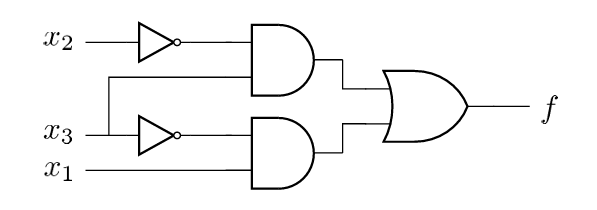
\includegraphics[scale=0.6]{logicgate2025-03-10.png}
\end{center} 
    A good indication of the \important{cost} of a logic circuit is the total number of \textbf{gates} and the \textbf{input} to the gates in the circuit.
    \begin{itemize}
        \item For the design above, the cost $ = 5 + 1 + 1 + 2 + 2 + 2 = 13$ where $5$ is the total gates, the one's are the NOT, $2$'s are the AND and OR.
            
    \end{itemize}
 \end{subparag}
 \begin{subparag}{Example PoS}
     Now we consider with product instead of a sum. Consider a function $f$ of $n = 3$ variables and the truth table below:
     \begin{align*}
         f(x_1, x_2, x_3) &= \prod(M_0, M_2, M_3, M_7) \\
                          &= \prod M(0, 2, 3, 7)
     \end{align*}
     \begin{align*}
         f(x_1, x_2, x_3) &= M_0 \cdot M_2 \cdot M_3 \cdot M_7 \\
                          &= (x_1 + x_2 + x_3)(x_1 + \overline{x_2} + x_3)(x_1 + \overline{x_2} + \overline{x_3})( \overline{x_1} + \overline{x_2} + \overline{x_3})
     \end{align*}
     And now using the Morgan's theorem:
     \begin{align*}
         f = \overbrace{f}^{=}= \overline{m_0 + m_2 + m_3 + m-7}
     \end{align*}
      \begin{center}
     \begin{tabular}{ccc|c}
         \hline
         $x_1$ & $x_2$ & $x_3$ & $f$ \\
         \hline
         \hline
         0 & 0 & 0 & 0 \\
         \hline
         0 & 0 & 1 & 1\\
         \hline
         0 & 1 & 0 & 0 \\
         \hline
         0 & 1 & 1 & 0 \\
         \hline
         1 & 0 & 0 & 1 \\
         \hline
         1 & 0 & 1 & 1 \\
         \hline
         1 & 1 & 0 & 1 \\
         \hline
         1 & 1 & 1 & 0 \\
         \hline
     \end{tabular}
     \end{center}
     Which as you can see is the same as the one before, but now we only take the line with $0$ as a result.
     \\
     After some trick, we finally get the result:
     \begin{align*}
         f(x_1, x_2, x_3) =(x_1 + x_3)( \overline{x_2} + \overline{x_3})
     \end{align*}
     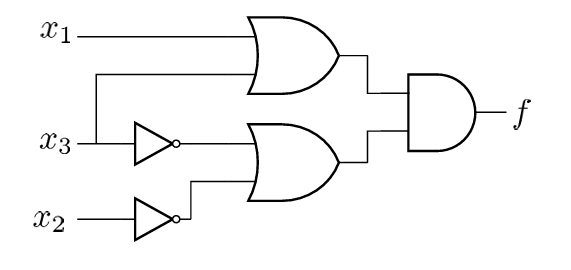
\includegraphics[scale=0.6]{gateAnd2025-03-10.png}
     Where the cost $ = 5 +  1 + 1 + 2 + 2 + 2 = 13$
 \end{subparag}
\end{parag}

\subsection{NANS and NOR logic Networks}
\begin{parag}{NAND and NOR gates}
    NAND and NOR gates can be used to build logic circuits:
    \begin{center}
        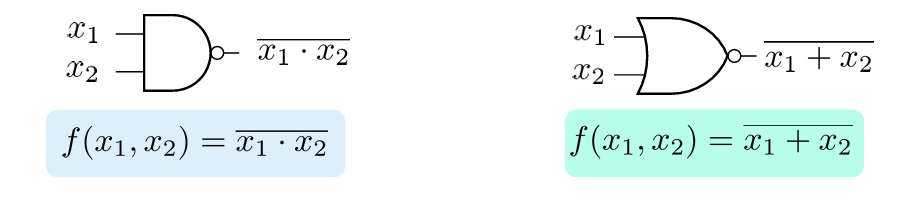
\includegraphics[scale=0.7]{NANDNOR2025-03-10.png}
    \end{center}
        NAND/NOR physical implementation is simpler (requires fewer transistor) and more efficient than AND/OR. In fact the AND and OR logic gates are implemented as NAND/NOR + not. How to de we that?:
        \begin{center}
            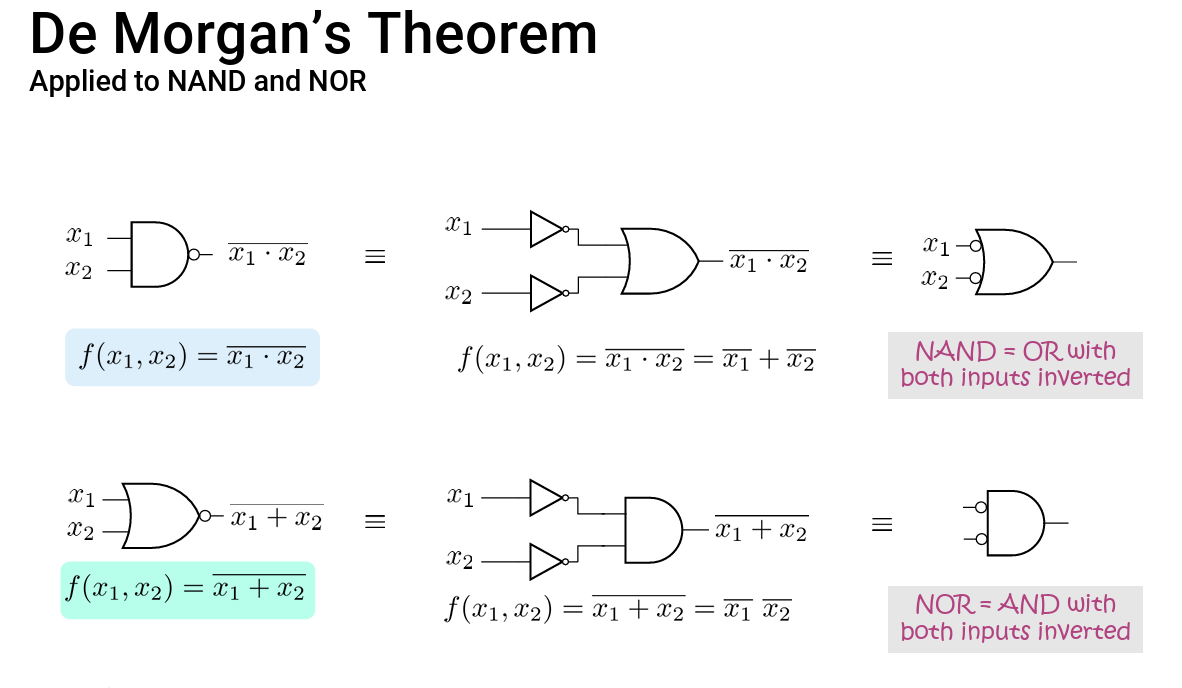
\includegraphics[scale=0.4]{morgantheoremgate2025-03-10.png}
        \end{center}

\end{parag}
\begin{parag}{NOT gate using NAND or NOR}
        According to Boolean theorems, $ \overline{x} = \overline{x \cdot x}$ and $ \overline{x} = \overline{x + x}$ which are the $NAND$ and the $NOR$:
\begin{center}
    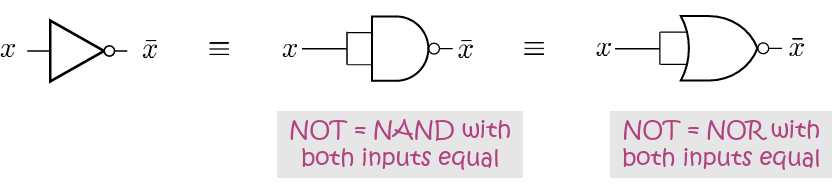
\includegraphics[scale=0.6]{notgatenandnor2025-03-10.png}
\end{center}
\begin{subparag}{How to implement a function}
    Now we try to implement the function $f$ in the $SoP$ form with $NAND$
    \begin{align*}
        f = x_2 + x_1 \overline{x_3}
    \end{align*}
    \textbf{Algorithm}: we start by applying double inversion and, then, the Morgan's theorem to simplify the expression.
    \\
    We have:
    \begin{align*}
        f &= x_2 + x_1 \overline{x_3} \\
          &= \overline{ \overline{ x_2 + x_1 \overline{x_3}}} \\
          &= \overline{ \overline{x_2} \cdot \overline{ x_1 \overline{ x_3}}}
    \end{align*}
    Which gives us:
    \begin{center}
        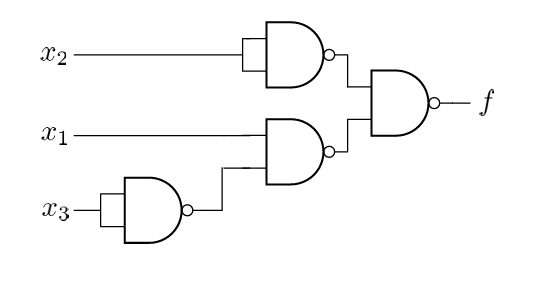
\includegraphics[scale=0.6]{gate22025-03-10.png}
    \end{center}
\end{subparag}

\end{parag}

\subsection{Incomplety definded Functions}
\begin{parag}{Incompletely defined function}
    …are Boolean functions where some input combinations are not specified because they don’t matter (e.g., they never occur), so the function does not need to define outputs for them
    \begin{itemize}
        \item Those input combinations are called \important{don't care conditions}
    \end{itemize}
    In logic optimization, don't care conditions can be assigned function value (output) either $0$ or $1$, to simplify the logic circuit
\end{parag}
\begin{parag}{Example}
    Imagine a lion's cage with an automated door control system including two sensors and a manual override switch.
    \textbf{Input}:
    \begin{itemize}
        \item \textbf{Sensor L} detects if the lion is inside ($1 =$ inside, $0 = $ outside=
        \item \textbf{Sensor T} detects if the trainer is inside ($1 = $ inside; $0 = $outside)
        \item \textbf{Override switch (S)}: The trainer can manually force the door open or closed irrespective of presence $(1 = $ override enabled; $0 = $ normal mode)
    \end{itemize}
    \textbf{Outputs}
    \begin{itemize}
        \item \textbf{Door control} $1$ = open, 0 = closed.
    \end{itemize}
    In this case with si that when $S = 1$ then L and $T$ doesn't matter, because the door will be open in any case.\\
    What we are doing here is this:
    \begin{align*}
        D = \overline{L}T \overline{S} + LT \overline{S} + \overline{L} \overline{T}S  = T \overline{S} + \overline{L} \overline{T}S
    \end{align*}
    Which have a cost of $ 3 + 7 = 10$\\
    However the result is the same by switching to
    \begin{align*}
        D = T + S
    \end{align*}
    In spoken english this is saying, the door can only be open if the switch is on or the trainer is inside and if neither of those two are true, then the door is closed. Here the cost is $1 + 2 = 3$
\end{parag}

\begin{parag}{Even and Odd detectors}
    Given the function $f = \overline{x_1}x_2 + x_1 \overline{x_2}$ which we called \important{Exclusive OR} or $XOR$ writted as $\oplus$:
    \begin{align*}
        f = x_1 \oplus x_2
    \end{align*}
    \begin{center}
        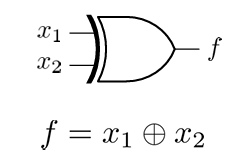
\includegraphics[scale=0.8]{xor2025-03-10.png}
    \end{center}
    On the other side for the $XNOR$ which is defined as $f = \overline{x_1} \overline{x_2} + x_1x_2$
    \begin{center}
        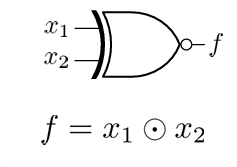
\includegraphics[scale=0.8]{xnor2025-03-10.png}
    \end{center}
    
\end{parag}
\begin{parag}{Number display}
    I skipped the previous slides (number display) because I am late but the goal was to write on a digital clock (with the 8 which as 7 lines that can be on or off) a value $(s_1, s_0)_2$ as a decimal number. To do so you have to do first a truth table depending of which line is on depending of the values, and the create a logic function from this truth table.
\end{parag}
\begin{parag}{Data selector}
    It is often helpful to choose \important{precisely one} from several inputs. A circuit performing data selection (a \important{multiplixer}) has one or more \important{select} inputs dedicated to determining which of the remaining inputs to pass to the output. \\
    For example, a three input multiplixer (also called $2$ to $2$ $MUX$):\\
    \textbf{Inputs}
    \begin{itemize}
        \item One \important{selection} signal $s$
        \item Two data \important{input} $x_1$ and $x_2$
    \end{itemize}
    When the selection signal is $s = 0$ the output becomes $f = x_1$ otherwise, the output becomes $f = x_2$\\
    To write this as a logical function:
\begin{align*}
    f(s, x_1, x_2) &= \overline{s}x_1 \overline{x_2} + \overline{s}x_1x_2 + s \overline{x}_1x_2 + sx_1x_2 \\
    \overline{s}x_1 ( \overline{x_2} + x_2) + s( \overline{x_1} + x_1)x_2 \\
    &= \overline{s}x_1 + sx_2
\end{align*}

\begin{subparag}{Remark}
  If there are $n$ data inputs to select from, how many select signals MUX requires?:
  \begin{align*}
      \left\lceil \log_2 n \right\rceil
  \end{align*}
  Because if we have two data, this give only one combination, 4 data two select signal, $2^2$, with eight data inputs, three select signals ($2^3$ combinations) and because we cannot take lower bound for data input that are not power of $2$, we have to take the ceiling.
  
\end{subparag}

\end{parag}





\lecture{8}{2025-03-14}{Arithmetic circuit}{}

\subsection{Adders}
\begin{parag}{Adders of two 1-bit binary}
Let us start from the simplest binary addition of one bit. The resulting sum is at most on two bits:
\begin{itemize}
    \item The rightmost bit is called $sum$(s)
    \item The leftmost bit is called $carry(c)$; it is produced as a carry-out when being a both bits being added are logical one
\end{itemize}
The goal is to create an addition with boolean arithmetic. Let us create a truth table:
\begin{center}
    \begin{tabular}{cccc}
        $x$ & $y$ & $s$ sum & $c$ carry \\
        \hline
        0 & 0 &0&0 \\
        0 & 1 & 1 & 0\\
        1 &0 &1&0\\
        1&1&0&1
\end{tabular}
\end{center}
we can as seen here, use one expression when the output is $1$ for the sum and another when the output is $1$ for the carry:
\begin{align*}
    s = \overline{x}y + x \overline{y} = x \oplus x
\end{align*}
For the carry:
\begin{align*}
    c = xy
\end{align*}

Which gives us the digital logic circuit:
\begin{center}
    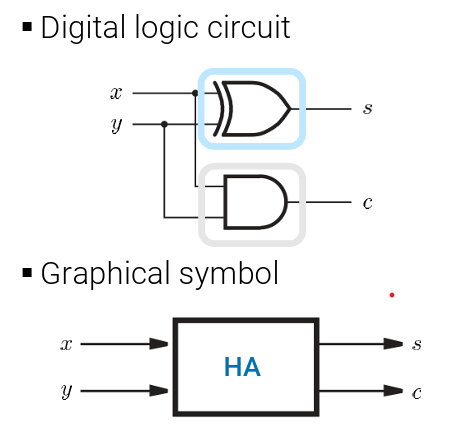
\includegraphics[scale=0.7]{12025-03-14.png}
\end{center}


\end{parag}
\begin{parag}{Addition of two $n$ bit binary number}
    A binary $n$-bit adder has two operands $0 \leq x, y \leq 2^n - 1$ and a carry in $c_{in} \in \{0 1\}$ as inputs, and produces as outputs:
    \begin{itemize}
        \item sum $0 \leq s \leq 2^n -1$
        \item Carry out $c_{out} \in \{0, 1\}$ such that:
            \begin{align*}
                x +  y + c_{in} = 2^nc_{out} + s
            \end{align*}
    \end{itemize}
    The solution to the above equation is:
    \begin{align*}
        s = (x + y + c_{in}) \mod 2^n
    \end{align*}

    Then we get for the carry:
    \begin{align*}
        c_{out} = \begin{cases}
            1 \text{ if } (x + y + c_{in}) \geq 2^n \\
            0 \text{ otherwise }
        \end{cases}
        = \lfloor  \frac{x + y + c_{in}}{2^n}\rfloor
    \end{align*}
    It is \important{impractical} to start from the truth table for $n$bit addition.
\end{parag}
\begin{parag}{Iterative approach}
    For the iterative algorithm:
    \begin{itemize}
        \item Add each pair of bits at the position $i, o \leq i \leq n$
        \item The addition at the bit position $i$ needs to include a carry-in at the position $i$ (i.e., carry out from the position $i-1$); it also generates a carry-in for the position $i + 1$
    \end{itemize}
    The $1$ bit adder reduces to a primitive module called \important{full-adder (FA)} with three binary inputs and two binary outputs such that:
    \begin{align*}
        x_i + y_i + c_i = 2c_{i+1} + s_i
    \end{align*}
\end{parag}
\begin{parag}{Full adder:}
    The goal now is to build the truth table for those outputs $s_i$ and $c_{i+1}$ from $x_i, y_i, c_i$:
    \begin{center}
    \begin{tabular}{ccccc}
        $x_i$ & $y_i$ & $c_i$ & $s_i$ & $c_{i+1}$ \\
        \hline
        0 & 0 & 0&0&0 \\
        0&0&1&1&0\\
        0&1&0&1&0\\
        0&1&1&0&1\\
        1&0&0&1&0\\
        1&0&1&0&1\\
        1&1&0&0&1\\
        1&1&1&1&1
    \end{tabular}
    \end{center}
    
    With the logical expression:
    \begin{align*}
        s_i &= \overline{x_i} \overline{y_i}c_i + \overline{x_i}y_i \overline{c_i} + x_i \overline{y_i} \overline{c_i} + x_iy_ic_i \\
            &= (x_iy_i + \overline{x_i} \overline{y_i})c_i + ( \overline{c_i}y_i + x_i \overline{y_i}) \overline{c_i} \\
            &= \overline{(x_i \oplus y_i)} c_i + (x_i \oplus y_i) \overline{c_i} = x_i \oplus y_i \oplus c_i
    \end{align*}
    And for $c_{i+1}$:
    \begin{align*}
        c_{i+1} &= \overline{x_i}y_ic_i + x_i \overline{y_i}c_i + x_iy_i \overline{c_i} + x_iy_ic_i \\
                &= ( \overline{x_i}y_i + x_i \overline{y_i})c_i + x_iy_i( \overline{c_i} + c_i) \\
                &= (x_i \oplus y_i)c_i + x_iy_i
    \end{align*}
    With give us:
    \begin{align*}
        c_{i+1} = x_iy_i + x_ic_i + y_ic_i
    \end{align*}
    \begin{subparag}{Example}
        Let us create a full-adder from a half adders:\\
        \begin{itemize}
            \item Half adder:
                \begin{align*}
                    s = \overline{x}y + x \overline{y} = x \oplus y\\
                    c = xy
                \end{align*}
            \item Full adder:
                \begin{align*}
                    s_i = x_i \oplus y_i \oplus c_i\\
                    c_{i+1} = (x_i \oplus y_i)c_i + x_iy_i
                \end{align*}
        \end{itemize}

        \begin{center}
            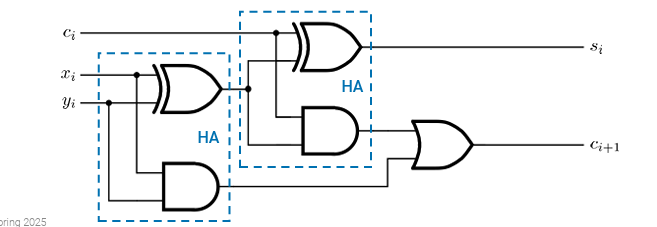
\includegraphics[scale=0.7]{22025-03-14.png}
        \end{center}
        Here we see the first result with the left \important{HA} and then go into a xor to the other adder
    \end{subparag}

    \begin{subparag}{Full adder}
        Here the logical circuit to the final logic expression:
        \begin{align*}
            s_i = x_i \oplus y_i \oplus c_i \\
            c_{i+1} = x_iy_i + x_ic_i + y_ic_i
        \end{align*}
        is:
        \begin{center}
            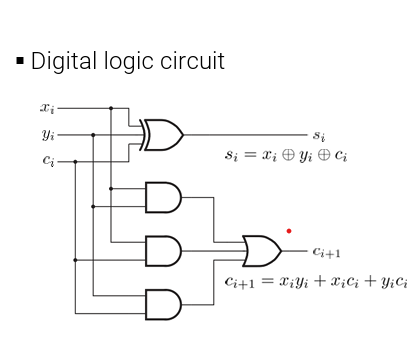
\includegraphics[scale=0.5]{32025-03-14.png}
        \end{center}
    With the graphical symbol     
        \begin{center}
            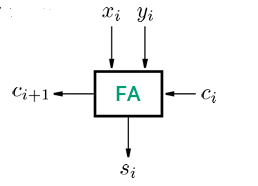
\includegraphics[scale=1.1]{42025-03-14.png}
        \end{center}
   \end{subparag}
   And the to be able to do an addition:
   \begin{itemize}
       \item Starting from the least significant digit, we add pairs of digits, progressing to the most significant digit
       \item Carry "ripples" through the adder stages
   \end{itemize}
   \begin{framedremark}
       There will be the same schema for the substraction juste below but I didn't put it here again to save the picture to document ratio. (but it is the slide 15)
   \end{framedremark}
   
\end{parag}
\begin{parag}{Substraction of two $1$ bit binary number}
    Subtraction generates two bits:
    \begin{itemize}
        \item \important{difference} (d), the result of the subtraction
        \item \important{borrow} (b), produced as a borrow out when the subtrahend is larger than minend
    \end{itemize}
\end{parag}
\begin{parag}{Subtraction of two n-bit unsigned number}
    it is \important{impractical} to start from the truth tables for $n$ bit substraction, if the exact same approach as the addition:
    \begin{itemize}
        \item Substract each pair of bits at the position $i, o \leq i < n$
        \item Subtraction at the bit position $i$ needs to include a borrow in at position $i$ (i.e., borrow out from the position $i - 1$); it also generates a borrow in position $i + 1$
    \end{itemize}

\end{parag}
\begin{parag}{Full subtractor}
    from the truth table:
    \begin{center}
    \begin{tabular}{ccccc}
        $x_i$ & $y_i$ & $b_i$ & $d_i$ & $b_{i+1}$ \\
        0&0&0&0&0\\
        0&0&1&1&1\\
        0&1&0&1&1\\
        0&1&1&0&1\\
        1&0&0&1&0\\
        1&0&1&0&0\\
        1&1&0&0&0\\
        1&1&1&1&1
    \end{tabular}
    \end{center}
   Which gives us:
   \begin{align*}
       d_i &= \overline{x_i} \overline{y_i} b_i + \overline{x_i}y_i \overline{b}_i + x_i \overline{y_i} \overline{b_i} + x_iy_ib_i\\
           &= ( \overline{x_i} \overline{y_i} + x_iy_i)b_i + ( \overline{x_i}y_i + x_i \overline{y_i}) \overline{b_i} = \overline{(x_i\oplus \overline{y_i})}b_i + (x_i \oplus y_i) \overline{b_i}\\
           &= x_i \oplus y_i \oplus b_i
   \end{align*}
   \begin{align*}
       b_{i+1} &= \overline{x_i} \overline{y_i} b_i + \overline{x_i}y_i \overline{b_i} + \overline{x_i}y_i \overline{b_i} + \overline{x_i}y_ib_i + x_iy_ib_i \\
    &= ( \overline{x_i} \overline{y_i} b_i + \overline{x_i}y_ib_i) + ( \overline{x_i}y_i \overline{b_i} + \overline{x_i}y_ib_i) + ( \overline{x_i}y_ib_i + x_iy_ib_i) \\
    &= \overline{x_i}b_i + \overline{x_i}y_i + y_ib_i
   \end{align*}
   With the same principle to the $n$bit ripple carry subtractor:
\begin{center}
    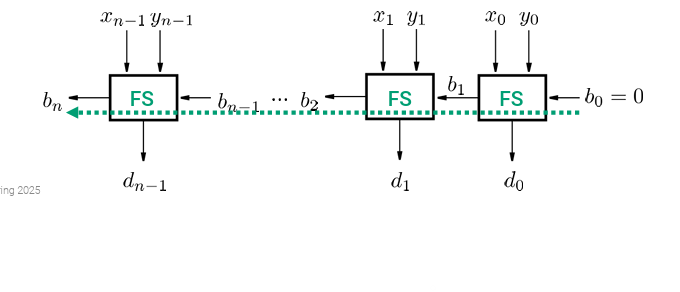
\includegraphics[scale=0.8]{52025-03-14.png}
\end{center}

   
   
\end{parag}
\begin{parag}{Adders-Subtractors in two's complement}
    Recall that subtracting two numbers in two's complement format requires using the two's complement of one operand:
    \begin{align*}
        X - Y = X + \overline{Y} + 1
    \end{align*}
    where 
    \begin{itemize}
        \item $ \overline{Y}$ is obtained by complementing every bit of $Y$
        \item Assume a control signal $op$ determines which $op$eration to perfom ( $op = 0$ is addition and $op = 1$ is subtraction)
    \end{itemize}
If we now assume a control signal $op$ determines which operation to perform then we can create the function $f$:
\begin{align*}
    f ( X, Y) = \begin{cases}
        X + Y \text{ if } op = 0\\
        X + \overline{Y} + 1, \text{ otherwise}
    \end{cases}
\end{align*}

Which with some  boolean algebraic operations:
\begin{align*}
    f(X, Y) &= \overline{op}(X + Y) + op(X + \overline{Y} + 1) \\
            &= ( \overline{op} + op) X + \overline{op}Y + op \overline{Y} + op \\
            &= X + \overline{op}Y + op \overline{Y} + op \\
            &= X op \oplus Y + op
\end{align*}

\begin{center}
    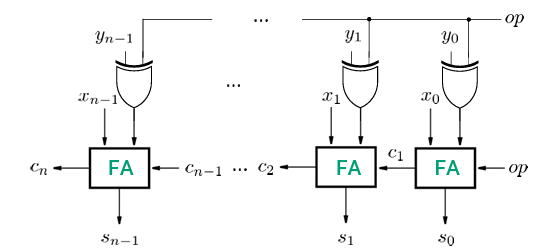
\includegraphics[scale=0.7]{62025-03-14.png}
    
\end{center}


\end{parag}

\subsection{Fast Adders}
\begin{parag}{Performance Matters}
Addition and subtraction are fundamental operations performed frequently. How quickly a result can be produced greatly impacts the system's performance. The performance is determined by the worst case delay.\\
The system's value is measured as a ratio:
\begin{align*}
    value = \frac{performance}{price}
\end{align*}
\begin{subparag}{Example}
    For example if we take the full adder (see the circuit there), There is a delay for each of the sum and the carry out, therefore for the worst case delay, we get:
    \begin{align*}
        t_{max} &= \text{max}(t(s_i), t(c_{i+1}))\\
                &= \text{max}(2t(XOR), t(XOR) + t(AND) + t(OR) \\
                &= 3 \text{ Gate Delays}
    \end{align*}

    
    
\end{subparag}
\end{parag}

\subsection{Shifting}
\begin{parag}{Barrel shifter}
    \begin{definition}
        A \important{barrel shifter} is a combinational logic circuit with $n$ data inputs $n$ data outputs, and a set of control inputs that specify how to shift data between the input and the output
    \end{definition}
    A barrel shifter inside a processor can typically specify
    \begin{itemize}
        \item \important{direction} of shift (left, right)
        \item \important{type} of shift (logical, arithmetic, circular/rotation)
        \item \important{amount} of shift (typically $0$ to $n-1$ bits)
    \end{itemize}
    implemented as a sequence of multiplexers (MUX), each shifting their input by twice as many positions as the previous MUX.
\begin{subparag}{How it works}
    A shifting is like you could imagine with only all bits going left or right and $0$ \textit{"replacing"} the one that get crushed.
\end{subparag}
\end{parag}



















\lecture{9}{2025-03-17}{Logisism}{}










\lecture{10}{2025-03-20}{intro to CAD and Verilog}{}
\begin{parag}{Previously on FDS}
\begin{itemize}
    \item We implemented $+/-$ arithmetic circuits using logic gates
        \begin{itemize}
            \item Basic building blocks: full adder and subtractor
            \item $N$-bit ripple carry adder in two's complement
        \end{itemize}
    \item Discovered the importante of circuit delay (Examples of critical path delay computation)
    \item Built fast adders: Carry-select adder
    \item Barrel shifters
        \begin{itemize}
            \item Used multiplexers to perform logic arithmetic shift
        \end{itemize}
\end{itemize}
\end{parag}

    \section{Computer Aided Design}
    \begin{parag}{Introduction to CAD tools}
        Logic circuit found in today's complex computing systems cannot be designed manually, Designers of logic circuits heavily rely on the availability of \important{computer-aided design (CAD)} tool:
   \begin{center}
       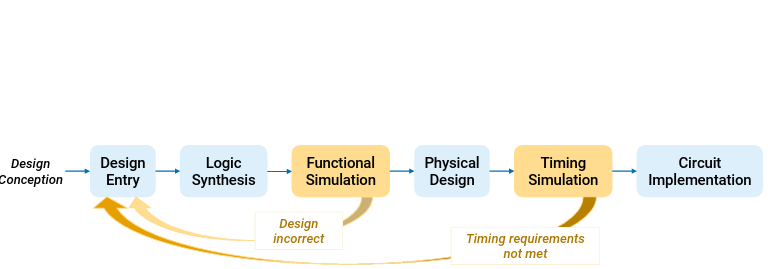
\includegraphics[scale=0.6]{12025-03-20.png}
   \end{center}
    
    \end{parag}
   \begin{parag}{Design Entry}
       Design entry is the starting point in the process of designing a logic circuit. The conception of what the circuit is supposed to do and the formulation of its general organization and structure. It the perfomrd by the designers without the guidance of CAD tools, it requires experience and intuition.
       \begin{subparag}{Approach $1$: Schematic capture}
           The goal here is to draw the logic gates and interconnecting them with writes, schematics tools provide libraries of gates and other circuit components.
           \begin{itemize}
               \item \important{Hierachical design}: Subcircuits previously created can be represented as graphical symbols and included (reused) in the schematic
           \end{itemize}
           
       \end{subparag}
       \begin{subparag}{Approach $2$: Hardware description language}
           An HDL is similar to a typical computer programming language exept that an HDL is used to describe hardware rather than a program to be executedd on a computer\\
           Mainstram HDL languages supported by vendors of digital hardware technology annd officially endorsed as IEEE standards:
           \begin{itemize}
               \item \important{Verilog HDL (cs-173)} and VHDL
           \end{itemize}

       \end{subparag}
       
   \begin{subparag}{HDL vs. Schematic capture}
       HDL's supported by many companies: no need to change the design from one company to another $ \implies$ Easy \important{portability}.\\ 
       Design entry means writing verilog source code, the code is plaint text which make it easy to include in the documentation $ \implies$ \important{Easy sharing and reuse}.\\
       Similar to schematic capture, HDLs support \important{hierachical design}\\
       HDL source can be \important{combined} with schematic capture (e.g., a subcircuit)
   \end{subparag}
   \end{parag}
    \begin{parag}{Functional simulation}
        A circuite described in the form of logic function can be simulated to verify that it will work as expected.\\
        Functional simulators assume the logic functions will be implement with \important{perfect gates (zero-delay model)}\\
       For the sequence of \important{inputs specified by the designers}, the simulator evaluates the circuit outputs and produces the results (e.g., \important{timing waveforms}) to be analyzed by the designers. Most often the result of this is a time diagram.
    \end{parag}
    
    
    \begin{parag}{Physical Design}
        \important{Mapping} a circuit described in the form of logic expression into a realization that uses logic gates or other hardware components available\\
        \important{Placement} Determine the absolute and relative location of the hardware components on physical chip\\
        \important{Routine} Determine the location and shape of the wiring connections that have to be made between the inputs and outputs of the hardware components to connect them appropriately.
    \end{parag}
    
    
   \begin{parag}{Timing simulation}
       Real circuits cannot perform their function with zero delay\\
       \important{llogic propagation delay}: Logic element need time to generate a valid output whenever there are changes in the value of their inputs\\
       \important{Wire propagation delay}
   
   \end{parag}
   
   \begin{parag}{Circuit implementation}
       Having ascertained that the circuit meets all desired requirements, the circuit is ready to be implemented on an actual chip\\
       \textbf{Option ahead}
       \begin{itemize}
           \item Chip fabrication (+ highest performance - extremely expensive)
           \item Chip configuration (+ flexible, + affordable, - lower performance)\\
    If a programmable hardware device is used as a baseline, the desired logic functionality can be implemented by simply reprogramming the device configuration
       \end{itemize}
   
   \end{parag}
   
    \subsection{Verilog}
    \begin{parag}{Bried history of verilog}
        \begin{itemize}
            \item HDLs were introduced in the mid 1980s as languages for describing the behavior of a logic circuit
            \item Verilog was invented by Phil Moorby and Prabhu 
                \begin{itemize}
                    \item A propriety language owned by Gateway design automation
                \end{itemize}
        \end{itemize}
    
    \end{parag}
    
   \begin{parag}{Modeling of digital circuits in verilog}
       A logic circuit is specified in the form of a \important{module}
       \begin{subparag}{Option $1$: Structural modeling}
           Gate-level modeling: Using verilog constructs to describe the structure of the circuit in terms of \important{circuit elements}, such as logic gates\\
           A larger circuit is defined by writing code that instantiates the 
           
       \end{subparag}
   
   \end{parag}
    
   \begin{parag}{Structural Modeling with logic gates}
       In structural modeling, predefined modules that implement basic logic gates are used\\
       Logic gate instantiation statement:
       \begin{center}
           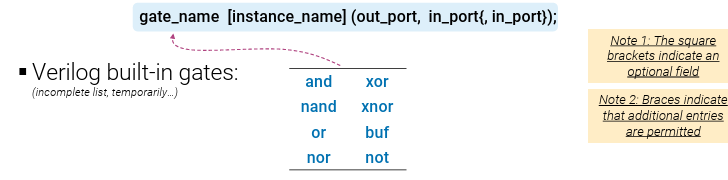
\includegraphics[scale=0.8]{22025-03-20.png}
       \end{center}

       \begin{subparag}{Example}
           Recall logic gate instantion statement:
           \begin{center}
               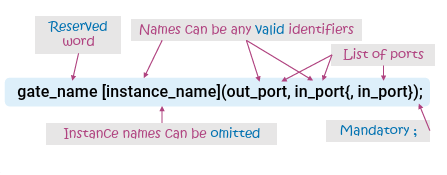
\includegraphics[scale=0.6]{32025-03-20.png}
           \end{center}
           
           
       \end{subparag}
       

   
   \end{parag}
   
      \begin{parag}{Verilog Syntax}
          \begin{subparag}{Names}
             \begin{itemize}
                 \item 
              Must start with a letter
          \item Can contain any letter, number, "\_"
             \end{itemize} 
          \end{subparag}
      
      \end{parag}
     
      \begin{parag}{Modules in verilog}
          Acircuit or subcircuit described with verilog code is a \important{module}. Module has a name, inputs, and outputs, referred to as its \important{prots}
          \begin{center}
              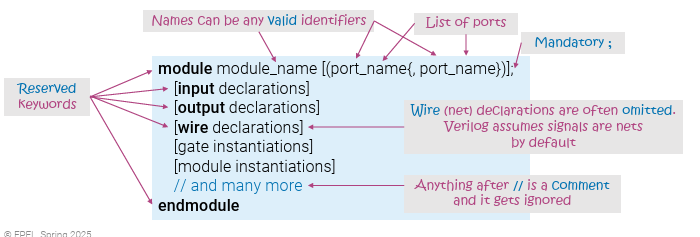
\includegraphics[scale=0.5]{42025-03-20.png}
          \end{center}
          
      
      \end{parag}
      
      
      \begin{parag}{Full adder in verilog}
          \begin{center}
              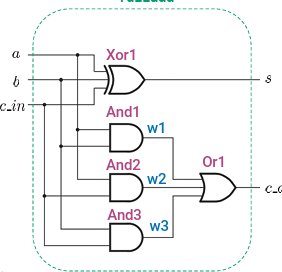
\includegraphics[scale=0.7]{52025-03-20.png}
          \end{center}
         \begin{subparag}{Algorithm}
             \begin{itemize}
                 \item Name your circuit
                     \begin{itemize}
                         \item That will be the name of your verilog module
                     \end{itemize}
                 \item Label all inputs and outputs
                     \begin{itemize}
                         \item Those will be the input and output port names of your verilog module
                             
                     \end{itemize}
                 \item Label all logic gates
                     \begin{itemize}
                         \item Those will be the names of your gates instances
                         \item same gate type can be instanciated multiple times, provided the instance name is unique
                     \end{itemize}
                 \item Label all internal nets
                     \begin{itemize}
                         \item Those will be the names of the wires in your Verilog module
                     \end{itemize}
             \end{itemize}
             
         \end{subparag} 
     \begin{subparag}{Concrete code}
         Here is how the code of the full adder would look like:
         \begin{center}
             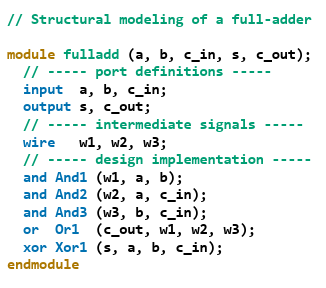
\includegraphics[scale=1]{62025-03-20.png}
         \end{center}
         
         
     \end{subparag} 
      \end{parag}
      \begin{parag}{Subcircuits in Verilog}
          A verilog module can be included as a subcircuit in another module. Modules should be defined in the same source file, in any order (or the verilog compiler must be told where each module is located).
     \textbf{Module instantiation statement } 
     \begin{center}
         \begin{align*}
             \text{module\_name instance\_name(.port\_name ([expression])\{,.port\_name(]expression])\});}
         \end{align*}
         
     \end{center}
    \begin{subparag}{Example}
        For example if we take the full add module created earlier and want to structure a Four-bit ripple Carry Adder, it would gives us:
        \begin{center}
            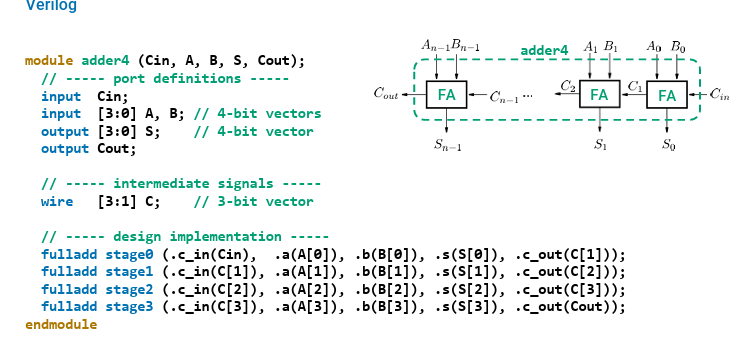
\includegraphics[scale=0.7]{72025-03-20.png}
            
        \end{center}
        
        
    \end{subparag} 
      \end{parag}
      
      

\lecture{11}{2025-03-24}{tri-state drivers}{}
\subsection{Tri-State Drivers}
\begin{parag}{Multiple gates driving same inputs}
    Imagine having two logic gate wanting to drive an input of a third logic gate.\\
    The issue here is the logic gates outputs should not be directly connected.
    \begin{itemize}
        \item If one gate forces '1' while the other forces '0', a low resistance path between the power supply and the ground would be created, and the resulting current would be high. We call that situation a \important{short circuit}.
    \end{itemize}
    \textbf{Solution}: Insert MUXes or tri-state drivers on the conflicting signal paths.
\end{parag}
\begin{parag}{Tris State Drivers}
    A tri-state driver has a data input, an output, and an \important{enable} input:
    \begin{center}
        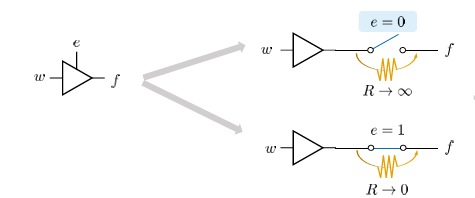
\includegraphics[scale=0.7]{12025-03-24.png}
    \end{center}
    The resulting output for this is:
    \begin{center}
    \begin{tabular}{cc|c}
        $e$ & $w$ & $f$ \\
        \hline
        \hline
        $0$ & $0$ & Z\\
        $1$ & $1$ & Z\\
        $1$ & $0$ & $0$\\
        $1$ & $1$ & $1$
    \end{tabular}
    \end{center}
    When the enable input is inactive, the output is eletrically disconnected from the data input; disconnected state is regerred to as \important{high impedance} state and usually denoted as $Z$ or $z$.
    
\begin{subparag}{Example}
    For example if we take a two gate outputs driving a wire:\\
    We need three tri-state drivers and then only one $e$ for the two tri state \important{BUT} inverted.
    \begin{center}
        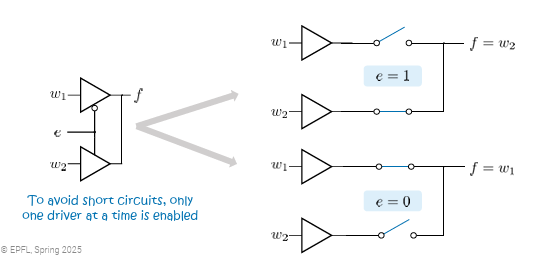
\includegraphics[scale=0.6]{22025-03-24.png}
    \end{center}
\end{subparag}
\end{parag}

\begin{parag}{Bus}
    Digital systems are commonly composed of several modules exchanging data by means of \important{common} set of interconnects (wires). \\
    The set of wires grouped under a common name is referred to as a \important{bus}
    \begin{framedremark}
        For example memory and CPU are connected with a Bus to exchange information.
    \end{framedremark}
    
    \begin{itemize}
        \item Bus receives data from several modules (one at a time) and brings that data to the inputs of other module
        \item Buses are typically $n$-bit wide, where $n > 1$
        \item Example: an $n$-bit bus DATA group $n$ wires each carrying one signal
            \begin{align*}
                DATA[0], \dots DATA[n-1
            \end{align*}
        \item In Verilog, $n$-bit and $1$-bit signals are called \important{vectors} and \important{scalars} respectively
    \end{itemize}
    This is a situation and we want to be able to implementing it.
\end{parag}
\begin{parag}{Implementing a Bus with MUXes}
    \begin{center}
        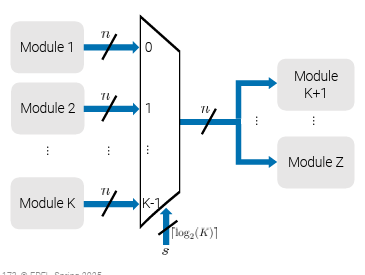
\includegraphics[scale=0.7]{42025-03-24.png}
    \end{center}
    \begin{itemize}
        \item The multiplexer takes $K$ ($k \geq 2$) n-bit data inputs and an $ \lceil \log_2 (K) \rceil$-bit select signal $s$ to select which of the inputs to pass to the output.
        \item An additional circuit that controls the activation of the \important{select} signals is typically present (which is not implemented here)
    \end{itemize}
    \begin{framedremark}
        When we have $k$ the number of select input is defined as $ \log_2(K)$,  and we rounded it up because it is defined the $2^{ \text{number of bit}}$ therefore if you take $2^{s} = K$ 
    \end{framedremark}
    
\end{parag}
\begin{parag}{Implementing a BUS with Tri-state Drivers}
    \begin{center}
        \includegraphics[scale=0.7]{52025-03-24.png}
    \end{center}
    \begin{itemize}
        \item \textbf{Only one} of the enable signals is \textbf{active} at a time so that short circuits are avoided.
        \item An additional circuit that controls the activation of the \textbf{enable} signals is typically present. (which is not implemented here)
    \end{itemize}
   
\end{parag}
\begin{parag}{Verilog Built-In Gates}
    Here is a complete list of the built in gate:
    \begin{itemize}
        \item \textbf{bufif} is a tri-state buffer
        \item \textbf{notif} is a tri-state inverter
    \end{itemize}
    \begin{center}
    \begin{tabular}{ccc}
        \hline
        and & xor & bufif0\\
        nand & xnor & bufif1\\
        or & buf & notif0\\
        nor & not & notif1
    \end{tabular}
    \end{center}
\end{parag}
\begin{parag}{Scalar  Signal Values}
    Verilog supports one-bit signal (scalars) and each individual signal can have one of the four values:
    \begin{center}
    \begin{tabular}{cc}
        \hline
        value & Meaning\\
        \hline
        $0$ & logic value $0$\\
        $1$ & logic value 1\\
        $z$ & or Z, tri-state (high impedance)\\
        $x$ & or $X$, unknown value or don't care
    \end{tabular}
    \end{center}
    Verilog support also multi-bit signal (vectors), therefore, we can specified the value of a vector by giving a constant of the form:
    \begin{align*}
        \text{[size]['radix]constant}
    \end{align*}
    Where \textit{size} is the number of bits in the constant
    \begin{center}
    \begin{tabular}{cc}
        d & decimal\\
        b & binary\\
        h & hexadecimal\\
        o & octal
    \end{tabular}
    \end{center}
   \begin{subparag}{Constants}
       If the size specifies more bits than are needed to represent the given constant, then in most casesm the constant is padded with zeors.
       \\
       the exceptions to this rule are when the first character of the constant is the either $x$ or $z$ , in which cases the padding is done using that value.
   \end{subparag}
    
\end{parag}

\begin{parag}{Concatenation Operator}
    Verilog concatenation operator $\{, \}$ allows vectos to be combined to produce a wider resulting vector:
    \begin{subparag}{Example}
        \begin{align*}
            \text{wire } [3:0] \text{ upper } = 4'b1100;\\
            \text{wire } [3:0] \text{ lower } = 4'b0011;\\
            \text{wire } [7:0] \text{ combined};
        \end{align*}
       The the result of the concatenation:
       \begin{align*}
           \text{assign } \text{ combined } = \{ \text{upper}, \text{lower}\}; \\
           = 8'b11000011
       \end{align*}
       
        
    \end{subparag}

\end{parag}
\begin{parag}{Parameters}
    parameter associate an identifier name with constant:
    \begin{subparag}{Example}
        \begin{center}
            parameter n = 4;
        \end{center}
    \end{subparag}

\end{parag}


\begin{parag}{Nets}
    Nets represent connections between circuit components, it doesn't store values, but transmit the signals. The wire are like a subclass of nets, the most common net types are $wire$ and $tri$. A wire is used to connect an output of one logic element in a circuit to an input of another logic element
    \begin{subparag}{Tri}
        The \important{tri} type denotes tri-state connections;\\
           tri nets are treated the \important{same way} as the \important{wires}; serve to enhance \important{readability} 
    \end{subparag}
\end{parag}
\subsection{Behavioral Modeling}


\begin{parag}{Example}
For instance given an input, we can label every logic gate and wrap it up into a module for instance:
\begin{center}
    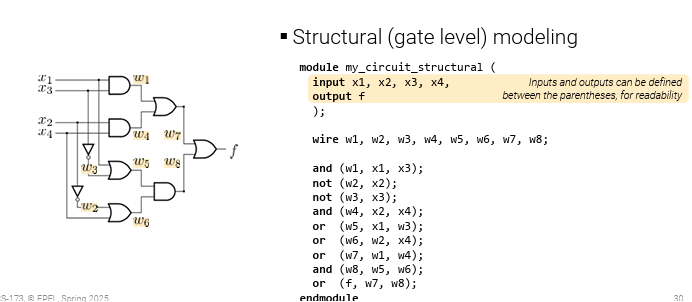
\includegraphics[scale=0.6]{12025-03-26.png}
\end{center}

\end{parag}
\begin{parag}{Behavioral modeling}

    Gate-level modeling becomes tedious for large circuit, the alternative is to use abstract expression and programming constructs to \important{ describe} the \textbf{behavior} of a logic circuit.
    \begin{center}
        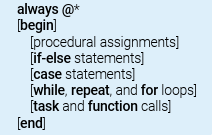
\includegraphics[scale=0.5]{22025-03-26.png}
    \end{center}
    All the operator can be use not only on the bits but on a vector.
    \begin{subparag}{Continuous assignments}
        The \important{assign} keyword provides a \important{continuous assignment for a signal}\\
        The term continuous stems from the use of Verilog in simulation of logic circuits.
        \begin{itemize}
            \item Whenever any signal on the right hand side of the assignment changes its value, the signal on the left-hand side will be re-evaluated
            \item \important{Continuous assignments are executed in parrallel}:\\
                Therefore, the order in which they appear in the code is irrelevant.
        \end{itemize}
        \begin{framedremark}
            for example, if we take $f = w7\; \mid\; w8$ whenever $w7$ or $w8$ change, $f$ \important{will be re-evaluated}.
        \end{framedremark}
    \end{subparag}
    
\end{parag}

\begin{parag}{Procedural statements}
    We can use all the \textit{"high"} level programming statements such as $if-else$, $case$, loops...\\
    hardware. However we kind of go away from the root and the "only" logic gate . Therefore, \\
    Procedural statements \important{must} be contained inside an \important{always}-block:
    \begin{itemize}
        \item Evaluated in the order given in the code.
    \end{itemize}
    To describe circuit behavior, variable are used instead of wires.
    \begin{itemize}
        \item For circuit modeling, variables of type $reg$ are used
    \end{itemize}
   
\end{parag}
\begin{parag}{Always block}
    The general format if a always block is given as:
    \begin{center}
        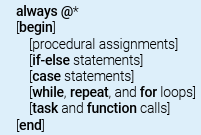
\includegraphics[scale=1]{32025-03-26.png}
    \end{center}
    \begin{framedremark}
        The square brackets indicate an optional field
    \end{framedremark}
    When multiple statements are included in the block, the begin and end keywords are needed.\\
    \textbf{always} write the (arobase)$^*$. 
\end{parag}
\begin{parag}{Full adder}
    For example if we wanted to created a full adder, we use a \textbf{case} statemants to describe the truth tables:
    \begin{center}
    \begin{tabular}{ccccc}
        x & y & $Cin$ & s & $Cout$\\
        0 & 0 & 0 & 0 & 0\\
        0 & 0 & 1 & 1 & 0\\
        0 & 1 & 0 & 1 & 0\\
        0 & 1 & 1 & 0 & 1\\
        1 & 0 & 0 & 0 & 0\\
        1 & 0 & 1 & 0 & 1\\
        1 & 1 & 0 & 0 & 1\\
        1 & 1 & 1 & 1 & 1 
    \end{tabular}
    \end{center}
Which gives us the following code:
\begin{center}
    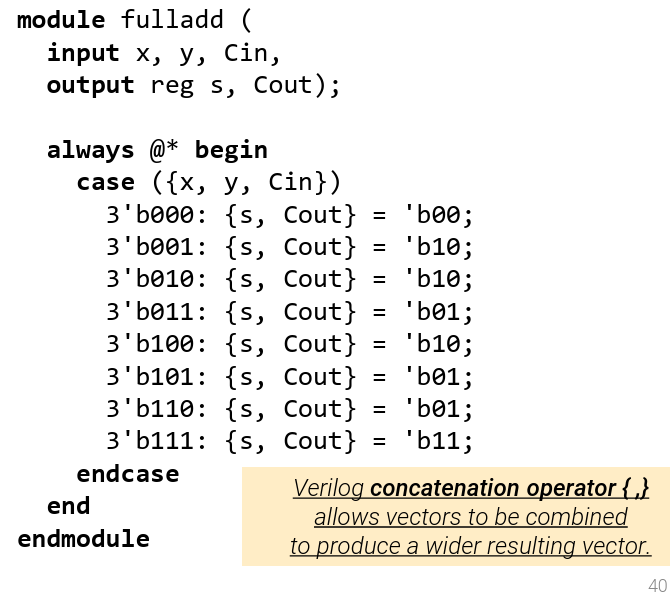
\includegraphics[scale=0.7]{42025-03-26.png}
    
\end{center}


\end{parag}




    \section{Transistors}
    There is too much schema for me to juste screenshot them and put it in the pdf, so until page 16 of the pdf Lecture -Digital Logic, Part VI, implementation technology.





\lecture{13}{2025-03-31}{this year mid term will be more difficult}{}
    \section{Sequential Logic}
    \begin{parag}{Example Application: Alarm System Control}
        Suppose that we wish to control an alaram system:
        \begin{center}
            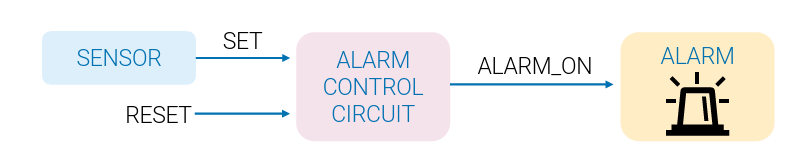
\includegraphics[scale=0.5]{12025-03-31.png}
        \end{center}
        If $ALARM\_ON = 1$, the alarm is activated; $ALARM\_ON = 0$, the alarm is deactivated.\\
        When the sense generate a positive voltage signal ($SET = 1$) in respone to some undesirable event, $ALARM\_ON$ becomes 1. \textbf{Once the alarm is triggered, it must remain active even if the sensor output returns to zero}. The alram is turned off by mans of a $RESET$ input. The circuit requires \important{a memory element} to remember that the alarm has to be active until the $RESET$ signal arrives.\\
        At this point in the course, we wouldn't be able to do so because we don't really have the sense of ``time''in combinational logic it is like a one-way function which is ``just used once''.
    \end{parag}
    \begin{parag}{Combinational vs. Sequential}
        Previously, we considered circuits where the value of each output depends solely and almost instantaneously on the values of signals applied to the inputs
        \begin{itemize}
            \item Refeerred to as \important{combinational circuits}
        \end{itemize}
        There exists another class of logic circuit in which the values of the outputs depend \textbf{not only on the} \important{present} valeus of the inputs \textbf{but  also on the} \important{past} behavior of the circuit.
    
        \begin{subparag}{Combinational circuits are \important{memoryless}}
            The outputs depends only on the present input.
        \end{subparag}
        \begin{subparag}{Sequential circuit}
            Outputs depend on the \textbf{present} and the \textbf{previous} inputs.
        \end{subparag}
        \begin{center}
            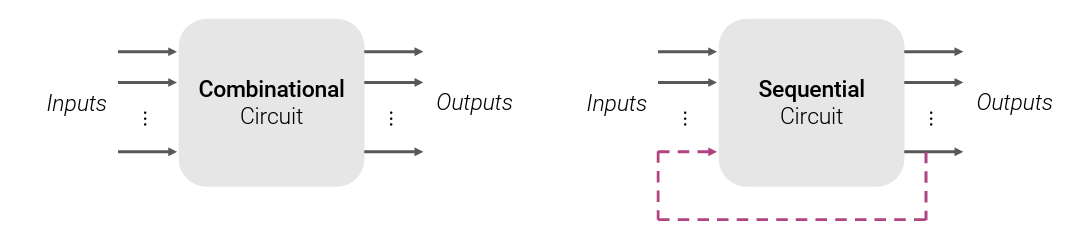
\includegraphics[scale=0.5]{22025-03-31.png}
        \end{center}
        
    \end{parag}
    \begin{parag}{Basic Memory Element}
            Here what we are looking for is a ``storage'' for the values of logic signal, it is this storage, or those stored values that \important{are the state of the circuit}. Therefore when the inputs change, the new input values either leave the circuit in the \important{same state} or cause it to change to a \important{new state}.\\
            Over time, the circuit changes through a \textbf{sequence of states} as a result of changes in the inputs.\\
        For instance, we can create a loop which inverts the input and re-inverts it etc... \\
        inverters with outputs connected to inputs:
        \begin{center}
            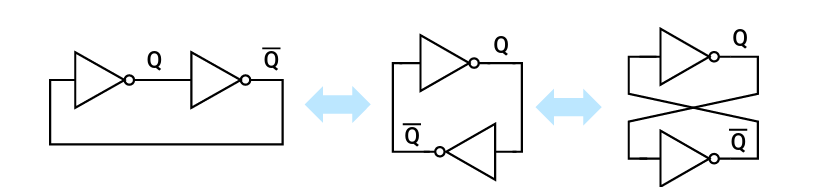
\includegraphics[scale=0.5]{32025-03-31.png}
        \end{center}
        
       However, this is not very practical because it stores a "given" value indefinitely, we cannot really access the value nor changes it so this is not really useful. What we want is to be able to access the element, therefore we need memory elements.
    
    \end{parag}
    \subsection{Memory Elements}
    \subsubsection{Latches}
    \begin{parag}{Set-Reset Latch with Reset priority}
        There is a memory element with NOR gates, \\
        Both NORs act as inverters in a bistable memory element:
        \begin{center}
            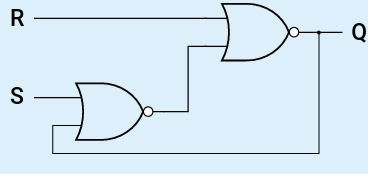
\includegraphics[scale=0.5]{42025-03-31.png}
        \end{center}
        \begin{definition}
            A table describing a sequential circuit behavior is called a \important{characteristic table}.
        \end{definition}
        How the next state changes in the function of the inputs \textbf{and} the previous state.
        \begin{center} \begin{tabular}{cc|c}$S$ & $R$ & $Q_{next}$ \\ \hline  0 & 0 &  \\ 0 & 1 &  \\ 1 & 0 & $f\left(S, R, Q\right)$ \\ 1 & 1 &  \end{tabular} \end{center} 
       \begin{subparag}{Latch}
           \begin{definition}
               Depending on the value of the output $Q$,  a latch be in one of the two states (S):
               \begin{itemize}
                   \item $S0: \; Q = 0$
                   \item $S1:\; = 1$
               \end{itemize}
               A state is a property of a memory element, State is defined by the logic value kept by the memory element $(Q)$.
           \end{definition}
       \end{subparag} 
       If we called the two NOR, $Q_b, Q_a$:
       \begin{align*}
           Q_b = \overline{S + Q_a}
       \end{align*}
       For the next $Q_a$ we get:
       \begin{align*}
           Q_{a, \; next} &= \overline{R + Q_b}\\
           &= \overline{R + \overline{S + Q_a}}\\
           &= \overline{R} \cdot (S + Q_a)\\
           &= \overline{R} \cdot S + \overline{R} \cdot Q_a = Q_{next}
       \end{align*}
       If we assume that  initially $Q_a = 0, Q_b = 1$ and \important{R is inactive (0)}.:
       \begin{itemize}
           \item When $S$ becomes $1$:
               \begin{itemize}
                   \item $Q_b$ becomes $0$, and $Q_a$ becomes $1$
               \end{itemize}
           \item While $S$ is $0$
               \begin{itemize}
                   \item $Q_a$ and $Q_b$ are complements of one another
                   \item Circuit state does not change (it is stable).
               \end{itemize}
       \end{itemize}
       
       However:
       \begin{itemize}
           \item Assume initially $Q_a = 0$, $Q_b = 1$
           \item $S$ is inactive
               \begin{itemize}
                   \item When $R$ becomes $1$:
                       \begin{itemize}
                           \item $Q_a$ becomes $0$, and $Q_b$ becomes $1$
                       \end{itemize}
                   \item While $R$ is $0$:
                       \begin{itemize}
                           \item $Q_a$ and $Q_b$ are complements of one another
                           \item Circuit state is stable
                       \end{itemize}
               \end{itemize}
       \end{itemize}
       Finally:
       \begin{itemize}
           \item Assume initially $Q_a = 0, Q_b = 1$,
           \item if both $S$ and $R$ are active:
               \begin{itemize}
                   \item $Q_a$ and $Q_b$ becomes $0$, both
               \end{itemize}
       \end{itemize}
       
       If we take the truth table:
       \begin{center}
       \begin{tabular}{cc|cc|cc}
           $S$ & $R$ & $ \overline{R} \cdot S$ & $ \overline{R} \cdot Q_a$ & $Q_{next}$ & $Q_{b, next}$ \\
           0 & 0 & 0 & $Q_a$ & $Q_a$ & $\overline{Q}_a$ \\
           1 & 0 & 1 & $Q_a$ & 1 & 0 \\
           1 & 1 & 0 & 0 & 0 & 0
       \end{tabular}
       \end{center}
       
       As you can see here, even when $S$ and $R$ are active, we still reset the output, this was a Latch we reset priority
        
    
    \end{parag}
    

    
    \begin{parag}{Set-reset latch with \important{Set} priotity}
      However it isn't always the best options to always have a reset priority, therefore we introduce also a Latch with a \important{Set} priority.
      \begin{center}
          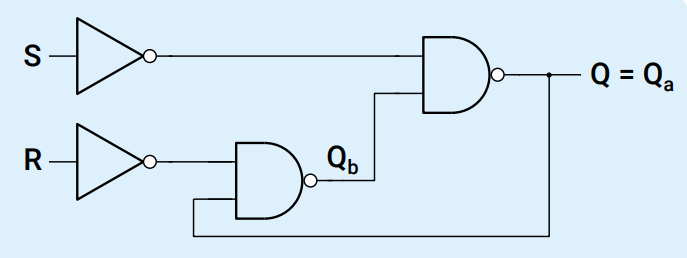
\includegraphics[scale=0.6]{12025-06-20.png}
      \end{center}
      \begin{align*} Q_{a, next} =  S + \overline{R}\cdot Q_a \end{align*}
      \begin{center} \begin{tabular}{cc|c|cc}$S$ & $R$ & $\overline{R}\cdot Q_a$ & $Q_{a, next}$ & $Q_{b, next}$ \\ 0 & 0 & $Q_a$ & $Q_a$ & $\overline{Q}_a$ \\ 0 & 1 & 0 & 0 & 1 \\ 1 & 0 & $Q_a$ & 1 & 0 \\ 1 & 1 & 0 & 1 & 1 \end{tabular} \end{center} 

      \begin{subparag}{Note}
         We usually try to avoid activating both $R$ and $S$.
      \end{subparag}
        
    \end{parag}
    
    \begin{parag}{Latches with a control signal}
        In practice, we want to  be able to control \important{when} state changes occur. To that purpose, we add a \textbf{control} signal.
        \begin{itemize}
            \item When active, it enables the latch to operate normally
            \item When inactive, it prevents states updates
        \end{itemize}
        
    \end{parag}
    \begin{parag}{$D$ latch}
        A D latch is a \important{Level sensitive} element, this means the change are allowed only when the control signal $C$ is active (at a high level).\\
        When the control signal is not active, the output $Q$ stays \textbf{unchanged}.\\
        \begin{subparag}{Personal note}
            A level sensitive element is a type of circuit components that whose behavior depends on the level of a control signal and not when it changes.\\
            For instance if you take a door, a sensitive level components would be:
            \begin{center}
                the door only opens when you press and \important{hold} a button
            \end{center}
            The button is the signal control here and opens the door \textbf{as long as the control signal is at a certain level}
           
            
        \end{subparag}
         \begin{center}
                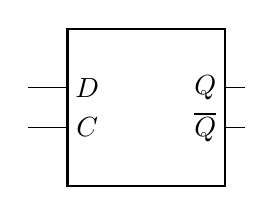
\begin{tikzpicture}
                    \draw[color=black, thick](0, 0) rectangle (2, 2);
                    \draw[](-0.5, 1.25) -- (0, 1.25) node at (0.25, 1.25) {$D$};
                    \draw[](2, 1.25) -- (2.25, 1.25) node at (1.75, 1.25) {$Q$};
                    \draw[](-0.5, 0.75) -- (0, 0.75) node at (0.25, 0.75){$C$};
                    \draw[](2, 0.75) -- (2.25, 0.75) node at (1.75, 0.75){$\overline{Q}$};
                \end{tikzpicture}
            \end{center}
            And the waveform is given as:
            \begin{center}
                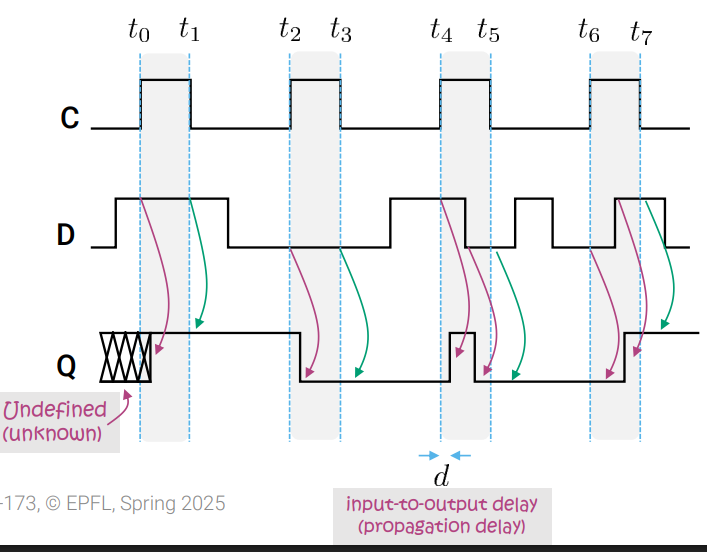
\includegraphics[scale=0.5]{22025-06-20.png}
            \end{center}
            
            
            
            
    \end{parag}
    
    \subsubsection{Flip-Flops}
    However, this issue with D latch is that as is it level sensitive, it changes more than one time while the control signal is active, in practice, limiting the duration of time when the state changes can occur is very desirable.\\
    Also, we want to memorize (keep) a state for a while and not allow it to change an unlimited number of times while the control signal is active (we will see why when we will do sequential logic)\\
    The goal it to allow the circuit to change state  only when the control signal \textbf{transition} (rising or falling edge)
    \begin{parag}{D Flip-Flop}
        A $D$ flip-flop is an \important{edge sensitive} memory element\\
        It responds to the changes at the input $D$ only when the controlling signal $C$ transitions
        
          \begin{center}
                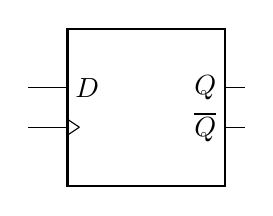
\begin{tikzpicture}
                    \draw[color=black, thick](0, 0) rectangle (2, 2);
                    \draw[](-0.5, 1.25) -- (0, 1.25) node at (0.25, 1.25) {$D$};
                    \draw[](2, 1.25) -- (2.25, 1.25) node at (1.75, 1.25) {$Q$};
                    \draw[](-0.5, 0.75) -- (0, 0.75) ;
                    \draw[](0, 0.85) -- (0.15, 0.75);
                    \draw[] (0, 0.65) -- (0.15, 0.75);
                    \draw[](2, 0.75) -- (2.25, 0.75) node at (1.75, 0.75){$\overline{Q}$};
                \end{tikzpicture}
            \end{center}
        
        \end{subparag}
        
        \begin{center}
            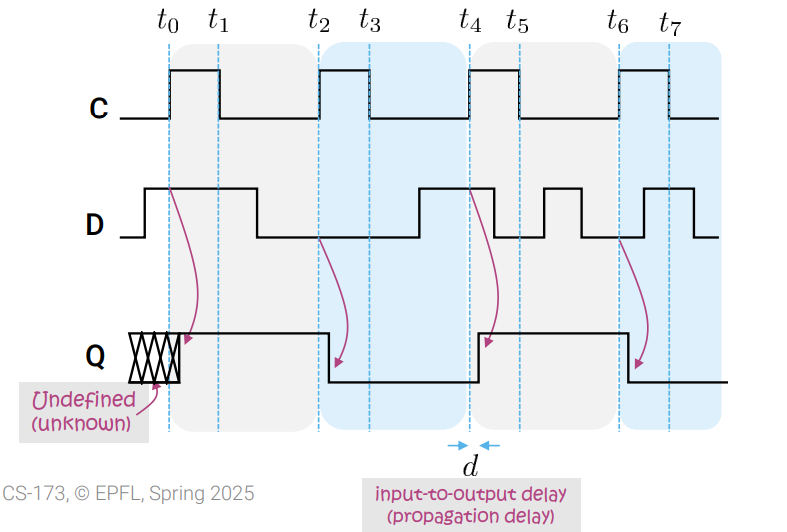
\includegraphics[scale=0.7]{32025-06-20.png}
        \end{center}
        
    \end{parag}
    
    
    

   \subsubsection{Clock}
   \begin{parag}{Clock signal}
       A Signal determine when the state changes occur is called \textbf{clock}.\\
       A clock is a periodic signal defined by its frequency (or period) and duty ratio \begin{framedremark}
       All digital system use clocks to synchronize state changes
       \begin{itemize}
           \item Typically, state changes are triggered by a rising edge of the clock.
       \end{itemize}
       
       \end{framedremark}

       
   \end{parag}
   \begin{parag}{Synchronous vs Asynchronous signal}
       \begin{itemize}
           \item A \important{synchronous signal} is one that is evaluated and updated only on the active edge (rising or falling) of the clock
           \item A \important{asynchronous signal} is one that immediately affects the output (the sate) regardless of the clock edge
       \end{itemize}
       
       
   \end{parag}
   
   
    
    
    


\end{document}
